% 学習結果説明（手順3b：設定温度の比較。用語集と図の見方）
% results フォルダで「lualatex 学習結果説明_手順3b.tex」を2回実行すると PDF を作り直せる（TeX Live の LuaLaTeX を使用）。
% 図は results/step3b/ の PNG を相対パスで読み込む。
\documentclass[paper=a4paper,fontsize=10.5pt,line_length=44zw,number_of_lines=38]{jlreq}
\usepackage[haranoaji]{luatexja-preset}
\usepackage{amsmath}
\usepackage{graphicx}
\usepackage{booktabs}
\usepackage{tabularx}
\usepackage{enumitem}
\usepackage{float}
\usepackage{xcolor}
\usepackage[hidelinks,bookmarksnumbered]{hyperref}
\graphicspath{{step3b/}}

\newcommand{\file}[1]{\texttt{\detokenize{#1}}}
\newcommand{\gd}{\dot{\gamma}}
\newcommand{\PII}{P3\_2}
\newcommand{\Tff}{T_{\mathrm{ff}}}
\newcommand{\Tset}{T_{\mathrm{set}}}
\newenvironment{termlist}{\begin{itemize}[label=・,leftmargin=1\zw,labelwidth=1\zw,labelsep=0pt,itemsep=0.4ex,topsep=0.6ex,parsep=0pt]}{\end{itemize}}
\newcommand{\term}[1]{\item \textbf{#1}：}
\newenvironment{points}{\begin{itemize}[label=$\triangleright$,leftmargin=1.5\zw,itemsep=0.3ex,topsep=0.5ex,parsep=0pt]}{\end{itemize}}
\newcommand{\pt}[1]{\item \textbf{#1}：}
\renewcommand{\arraystretch}{1.25}

\title{樹脂粘度モデル開発　手順3bの学習結果の説明\\[0.6ex]{\large 設定温度の比較：用語集とグラフの見方（機械学習・統計を初めて学ぶ人向け）}}
\author{}
\date{2026年10月13日}

\begin{document}
\maketitle
{\small\tableofcontents}

% =====================================================================
\section{この文書について}

この文書は、\file{results/step3b/} にある手順3bの結果（図と表）を、機械学習や統計を初めて学ぶ人でも読めるように説明したものです。手順3a・手順2の説明書（\file{学習結果説明_手順3a.pdf}・\file{学習結果説明.pdf}）と同じ形で、重なる用語は短く繰り返しています。

\begin{points}
\pt{対象の結果}\file{results/step3b/}：粘度の予測に、加熱シリンダの設定温度 $\Tset$ を入力として足すと、何が変わるかを調べた結果です（図 8 枚、CSV 7 個）。あわせて、流動先端温度 $\Tff$ と圧力 \PII\ が本当に要らないか、ショットごとの $\gd$ を使うか条件ごとの平均を使うかを比べました。
\pt{読み方}2章で何をしたかをつかみ、分からない言葉は3章の用語集で調べてください。4章で図の見方、5章で表の見方、6章で結果のまとめと、質問への答えを説明します。
\pt{数値について}文中の数値は、この文書を作った時点の results の表から取り出したものです。
\pt{元のノート}\file{01_機械学習コードフォルダ} の \file{手順3b_新データ_設定温度の比較.ipynb} です。ノートの先頭に使い方があり、「設定エリア」だけを直せば設定を変えられます。各節の最後に出る「判定」（\texttt{OK} と \texttt{★要確認}）の読み方は、3.4節にあります。報告書・発表資料用の高解像度のグラフ（せん断速度 ― 粘度）は、ノート11章のセルで作ります（4章の最後）。
\pt{記号表}記号・モデル名（B0T、R3 など）・列名の一覧は、\file{学習結果説明_記号表.pdf} にあります。
\pt{作り直し方}\file{results} フォルダで \texttt{lualatex 学習結果説明\_手順3b.tex} を2回実行すると、この PDF を作り直せます。
\end{points}

% =====================================================================
\section{何をしたか（概要）}

\subsection{目的}
これまでの手順で、粘度の予測に使える入力は「せん断速度 $\gd$」と「キャビティ厚み $H$」だとわかりました（手順3a）。圧力 $P3\_1$ は粘度の算出式そのものなので使えず、$\PII$ は効果が小さく、予測の場面で使いにくい値です。手順3bでは、次の4点を確かめました。

\begin{table}[H]
\caption{確かめた4つの点}
\begin{tabularx}{\linewidth}{@{}>{\raggedright\arraybackslash}p{9\zw}>{\raggedright\arraybackslash}p{19\zw}X@{}}
\toprule
点 & 確かめること & 見る場所 \\
\midrule
1 設定温度は要るか & $\Tset$ を入力に足すと、予測が良くなるか。190 ℃ と 230 ℃ の粘度の差を、実測どおりに出せるか。 & 図1・図5、表\ref{tab:eff}・\ref{tab:st} \\
2 $\Tff$ は要るか & 流動先端温度（実測値）を足すと、予測が良くなるか。（ユーザー決定：「あり」と「なし」の両方を、目で見て比べる） & 図1、表\ref{tab:sv_pp}・\ref{tab:sv_mix}・\ref{tab:st} \\
3 \PII\ は要るか & 圧力 \PII\ を足すと、予測が良くなるか。 & 同上 \\
4 $\gd$ の入れ方 & ショットごとの $\gd$ と、条件ごとの平均の $\gd$ のどちらを入力にするか。 & 図2・図7、表\ref{tab:noise} \\
\bottomrule
\end{tabularx}
\end{table}

あわせて、問題データ一覧の「感度確認」の条件（P02：190 ℃・0.5 mm・20 mm/s、P03：PP の 190 ℃・0.5 mm・320 mm/s）の影響を調べ、影響が大きければ、その条件だけを除いたデータファイルを新しく作る、という決まりに従って判断しました（表\ref{tab:sens}）。

\subsection{データ}
\begin{points}
\pt{データ}手順3aと同じです。5data（学習）と 3data（検証）は、条件が重ならず、合わせて 129 条件です。外れ値なしのファイルを主に使い、PP は、問題データ一覧の「除外」（厚み 1.5 mm・射出速度 3 mm/s の3条件）を除きます。学習は PP が 460 行（93 条件）、粉砕材混合 PP が 459 行（93 条件）、検証は PP が 95 行（33 条件）、粉砕材混合 PP が 101 行（36 条件）です。
\pt{圧力の単位}CSV の圧力は MPa です。Pa に直してから $\ln$ をとりました。
\end{points}

\subsection{比べたモデル}
目的変数（予測したい量）は、どのモデルも粘度の自然対数 $\ln\eta$ です。入力はすべて $\ln$ をとった値です（$\Tset$ は ℃ のまま。$\Tff$ は K で）。名前の付け方は、B 系が「ショットごとの $\gd$ を使う」、R 系が「条件ごとの平均の $\gd$ を使う（Rは Reference：設定値から見た形）」です。

\begin{table}[H]
\caption{比べた15のモデル（ln は自然対数）}
\begin{tabularx}{\linewidth}{@{}l>{\raggedright\arraybackslash}p{8\zw}X@{}}
\toprule
記号 & 種類 & 入力 \\
\midrule
L0・L0T & 線形回帰（基準） & $\gd$，$H$ ／ さらに $\Tset$ \\
B0 & GPR（ショットごと） & $\gd$，$H$ \\
B0T & GPR（ショットごと） & $\gd$，$H$，$\Tset$ \\
B0F・B0FT & GPR（ショットごと、$\Tff$ あり） & $\gd$，$H$，$\Tff$ ／ さらに $\Tset$ \\
B2・B2T & GPR（ショットごと、\PII\ あり） & $\gd$，$H$，\PII ／ さらに $\Tset$ \\
B2F・B2FT & GPR（ショットごと、$\Tff$・\PII\ あり） & $\gd$，$H$，$\Tff$，\PII ／ さらに $\Tset$ \\
R0 & GPR（条件ごとの値） & 条件平均の $\gd$，$H$ \\
R2 & GPR（設定値だけ） & 射出速度 $v$，$H$，$\Tset$ \\
R3 & GPR（条件ごとの値） & 条件平均の $\gd$，$H$，$\Tset$ \\
R3F & GPR（条件ごとの値、$\Tff$ あり） & 条件平均の $\gd$，$H$，$\Tset$，$\Tff$（条件平均） \\
R3P & GPR（条件ごとの値、\PII\ あり） & 条件平均の $\gd$，$H$，$\Tset$，\PII（条件平均） \\
\bottomrule
\end{tabularx}
\end{table}

GPR はすべて、ARD 付き Matern 5/2 カーネルに、\textbf{線形カーネル（DotProduct）}とノイズ項を足したものです（ユーザー決定：低速側への外挿のため）。R3 が、CLAUDE.md §6 の「比較用の通常の GPR」にあたります。

\subsection{データの分け方}
\begin{table}[H]
\caption{学習データとテストデータの分け方}
\begin{tabularx}{\linewidth}{@{}lX@{}}
\toprule
記号 & 分け方 \\
\midrule
S\_V & 5data で学習し、3data で検証する（射出速度の両端の外挿）。低速側（3・5 mm/s）と高速側（280・320 mm/s）に分けて評価する。 \\
S\_T & 5data の 190 ℃ と 230 ℃ だけで学習し、5data の 210 ℃ の全条件をテストする（設定温度の内挿。中間の温度を、両側から予測できるか）。 \\
S\_T3 & S\_T と同じ学習で、3data の 210 ℃ をテストする（温度の内挿に、速度の外挿が重なる）。 \\
S\_R1・S\_R2 & 従来の、行単位のランダム 20\%（S\_R1：Alldata、S\_R2：PP の 5data＋3data）。評価の甘さを見る。 \\
LOCO & 条件を1つずつ抜く交差検証（ハイパーパラメータは全データで決めて固定。近似）。 \\
\bottomrule
\end{tabularx}
\end{table}

\subsection{そのほかの設定}
\begin{points}
\pt{標準化と中心化}学習データだけで計算しました。
\pt{ハイパーパラメータ}最尤推定で、1組だけ求めました（最終候補の MCMC は手順3c）。ノイズ分散の下限は $10^{-6}$ です。
\pt{感度確認}問題データ一覧の P02・P03 を学習から除いて学習し直した結果と、外れ値ありのデータでの結果を並べました。
\pt{乱数}シードは 42 に固定しました。
\end{points}

% =====================================================================
\section{用語集}

手順3a・手順2の用語集になかったものを中心に、「・用語：説明」の形で並べました。

\subsection{温度とせん断速度の入れ方}
\begin{termlist}
\term{加熱シリンダ設定温度 $\Tset$}成形機に設定した樹脂の温度（190・210・230 ℃）。成形条件として事前に決まる値で、予測のときも指定できます。
\term{流動先端温度 $\Tff$}センサの間を流れている樹脂の先端の温度（実測値）。流れの速さで上下する、流れの「結果」の量です。
\term{ショットごとの $\gd$ と、条件ごとの平均の $\gd$}同じ条件で何度も成形すると、$\gd$ はショットごとに少しゆれます。そのゆれは、粘度のゆれと強く連動しています（相関 $-0.98$）。ショットごとの $\gd$ を入力にすると、GPR がこの連動を利用でき、ノイズ分散が極端に小さくなります（$5\times10^{-5}$ ほど）。条件ごとの平均を入力にすると、成形条件から見た「ほんとうのばらつき」が出ます。この文書では、前者を\textbf{ショットごと（shot）}、後者を\textbf{条件平均（cm。condition mean）}と呼びます。
\term{設定温度の効果（粘度の比）}同じ厚み・同じ $\gd$ で、190 ℃ の粘度が 230 ℃ の何倍か。実測は 1.07〜1.20 倍で、厚いほど大きくなります。モデルでは、他の入力はそのままで、$\Tset$ だけを 190 ℃ と 230 ℃ にして予測した粘度の比で表します。
\term{設定値と、測定値}射出速度・厚み・設定温度は、成形条件として決める「設定値」です。$\gd$・$\Tff$・\PII\ は、成形してから測る「測定値」で、事前には分かりません。
\end{termlist}

\subsection{評価に関する用語}
\begin{termlist}
\term{S\_T（中間温度のホールドアウト）}210 ℃ のデータを、学習から全部除いて、190 ℃ と 230 ℃ だけで学習し、210 ℃ を予測する検証。温度の影響を、補間で出せるかを見ます。
\term{内挿と外挿}手順3aの用語集と同じです。S\_T は温度についての内挿、S\_V は速度についての外挿、S\_T3 は両方が重なります。
\term{RMSE・被覆率・NLPD}手順3aの用語集と同じです。RMSE は予測の平均的な誤差（$\ln\eta$。0.05 なら粘度で約 5\%）、被覆率は 95\% 予測区間に実測が入った割合（0.95 が理想）、NLPD は予測の当たり具合と区間の適切さをまとめた指標（小さいほど良い）です。
\term{感度確認}ある条件を学習や評価から除いたとき、結果がどれだけ変わるかを見ること。変わりが大きい条件は、結果を左右しているので、扱いを決める必要があります。
\term{長さスケールの張り付き}GPR の長さスケールは、入力がどれだけ変わると出力が大きく変わるかの目安です。探索範囲の下限（0.01）に張り付くと、「その入力は、少しでも違えば、別物」とみなす（滑らかさを捨てる）ことになり、間の値を内挿できなくなります。設定温度のように水準が少ない入力で起きやすい現象です。
\term{線形カーネル（DotProduct）}手順3aの用語集と同じです。GPR に「直線的な傾向」を加え、学習範囲の外でも、傾きを延ばして予測できるようにします。
\end{termlist}

\subsection{ノートの「判定」の読み方}
ノートの各節の最後に、\texttt{>> 判定：OK} か \texttt{>> 判定：★要確認} が出ます。\texttt{OK} は、文の中に書いた基準を満たす（想定どおり）、\texttt{★要確認} は満たさない（想定と違う、または注意が要る）ことを表します。\texttt{★} が出ても、エラーではありません。結果を読むときに注意する点の目印です。この文書の6章で、主な \texttt{★} の意味を説明します。

% =====================================================================
\section{図の見方}

図ごとに、「何を示す図か」「軸と記号」「見るポイント」「今回の結果」の順に説明します。図のファイルは \file{results/step3b/} にあります。

% ---------------------------------------------------------------------
\subsection{図1：設定温度ごとの予測曲線（Tff・\PII\ の有無を目で比べる）}
\begin{figure}[H]
\centering
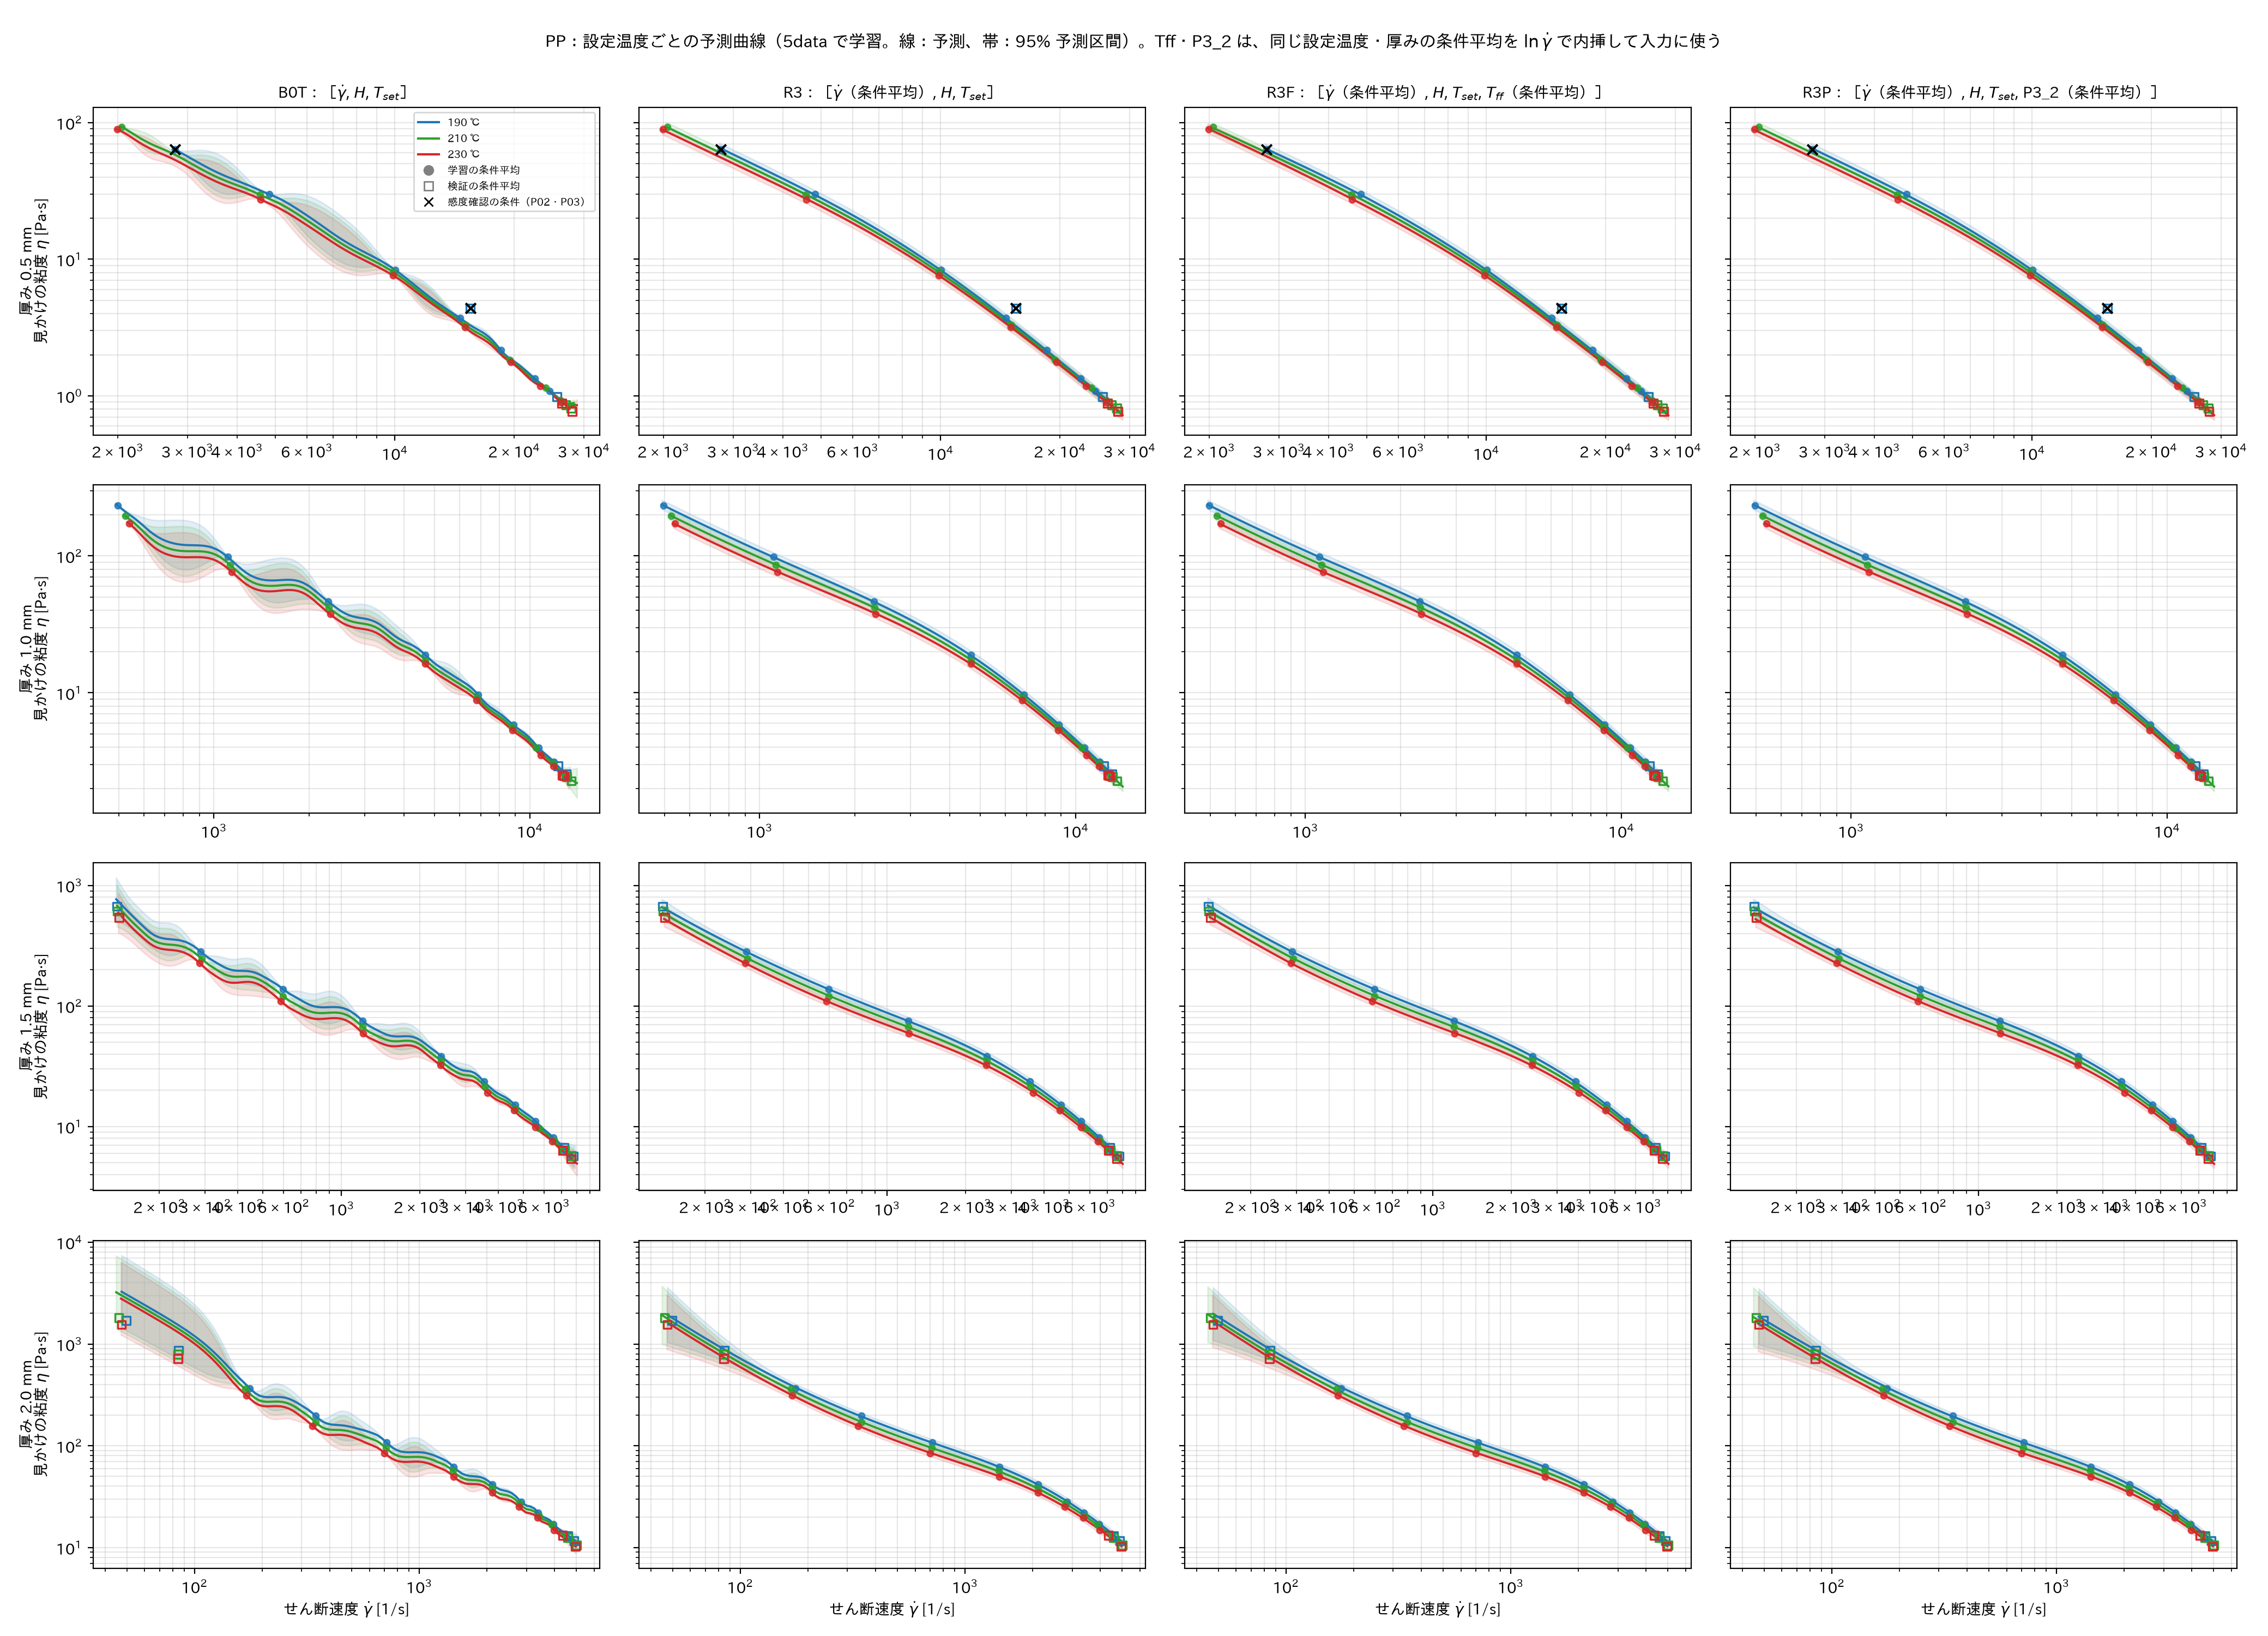
\includegraphics[width=\linewidth]{fig1a_tset_curves_PP.png}
\caption{PP：設定温度ごとの予測曲線（5data で学習。行：厚み、列：モデル）}
\end{figure}
\begin{points}
\pt{ファイル}\file{results/step3b/fig1a_tset_curves_PP.png}（PP）、\file{fig1b_tset_curves_MIX.png}（粉砕材混合 PP）
\pt{何を示す図か}5data で学習したモデルが、設定温度ごとにどんな粘度曲線を予測するかを、データと重ねた図です。$\Tff$ と \PII\ の「あり・なし」の違いを、グラフで確かめるための図です（ユーザー決定）。
\pt{軸と記号}横軸が $\gd$ [1/s]、縦軸が $\eta$ [Pa$\cdot$s]（どちらも対数軸）。行が厚み（0.5〜2.0 mm）、列がモデル（B0T：ショットごと、R3：条件平均、R3F：さらに $\Tff$、R3P：さらに \PII）。線の色が設定温度（青 190 ℃、緑 210 ℃、赤 230 ℃）、帯が 95\% 予測区間。塗りつぶしの丸が学習の条件平均、白抜きの四角が検証（3data）の条件平均、黒い×が感度確認の条件です。$\Tff$・\PII\ は、同じ設定温度・厚みの条件平均を $\ln\gd$ で内挿した値を入力にしています。
\pt{見るポイント}(1) 3 本の線が、温度の順（190 ℃ が上）に並ぶか。(2) 白抜きの四角（外挿の検証）が、線と帯に乗るか。(3) $\Tff$・\PII\ を足した列（R3F・R3P）が、R3 と違って見えるか。(4) 帯が、低速側で広がるか。
\pt{今回の結果}B0T（ショットごとの $\gd$）の線は、波打ち、帯の幅も場所で変わります。ショットごとの $\gd$ のゆれに合わせて、曲線を細かく曲げているためです。R3（条件平均）は、なめらかな線で、3 本が温度の順に並び、検証の白抜きの四角（外挿）にも乗ります。帯は、低速側（左端）で広がります。R3F（$\Tff$ あり）は、線の見た目は R3 とほぼ同じですが、これは、各線の $\Tff$ を、温度ごとの条件平均から与えているためです。$\Tset$ だけを変えて予測すると、粘度の比は PP で 1.00〜1.04、粉砕材混合 PP で 1.01〜1.05 と、ほとんど 1 です（実測は 1.08〜1.19、1.07〜1.19。表\ref{tab:eff}）。$\Tff$ は温度そのものを反映した値なので、入れると、温度の情報を $\Tff$ が受け持ち、$\Tset$ が使われなくなります。R3P（\PII\ あり）は、R3 と見分けがつきません。
\end{points}

% ---------------------------------------------------------------------
\subsection{図2：検証データ（S\_V）のパリティ図}
\begin{figure}[H]
\centering
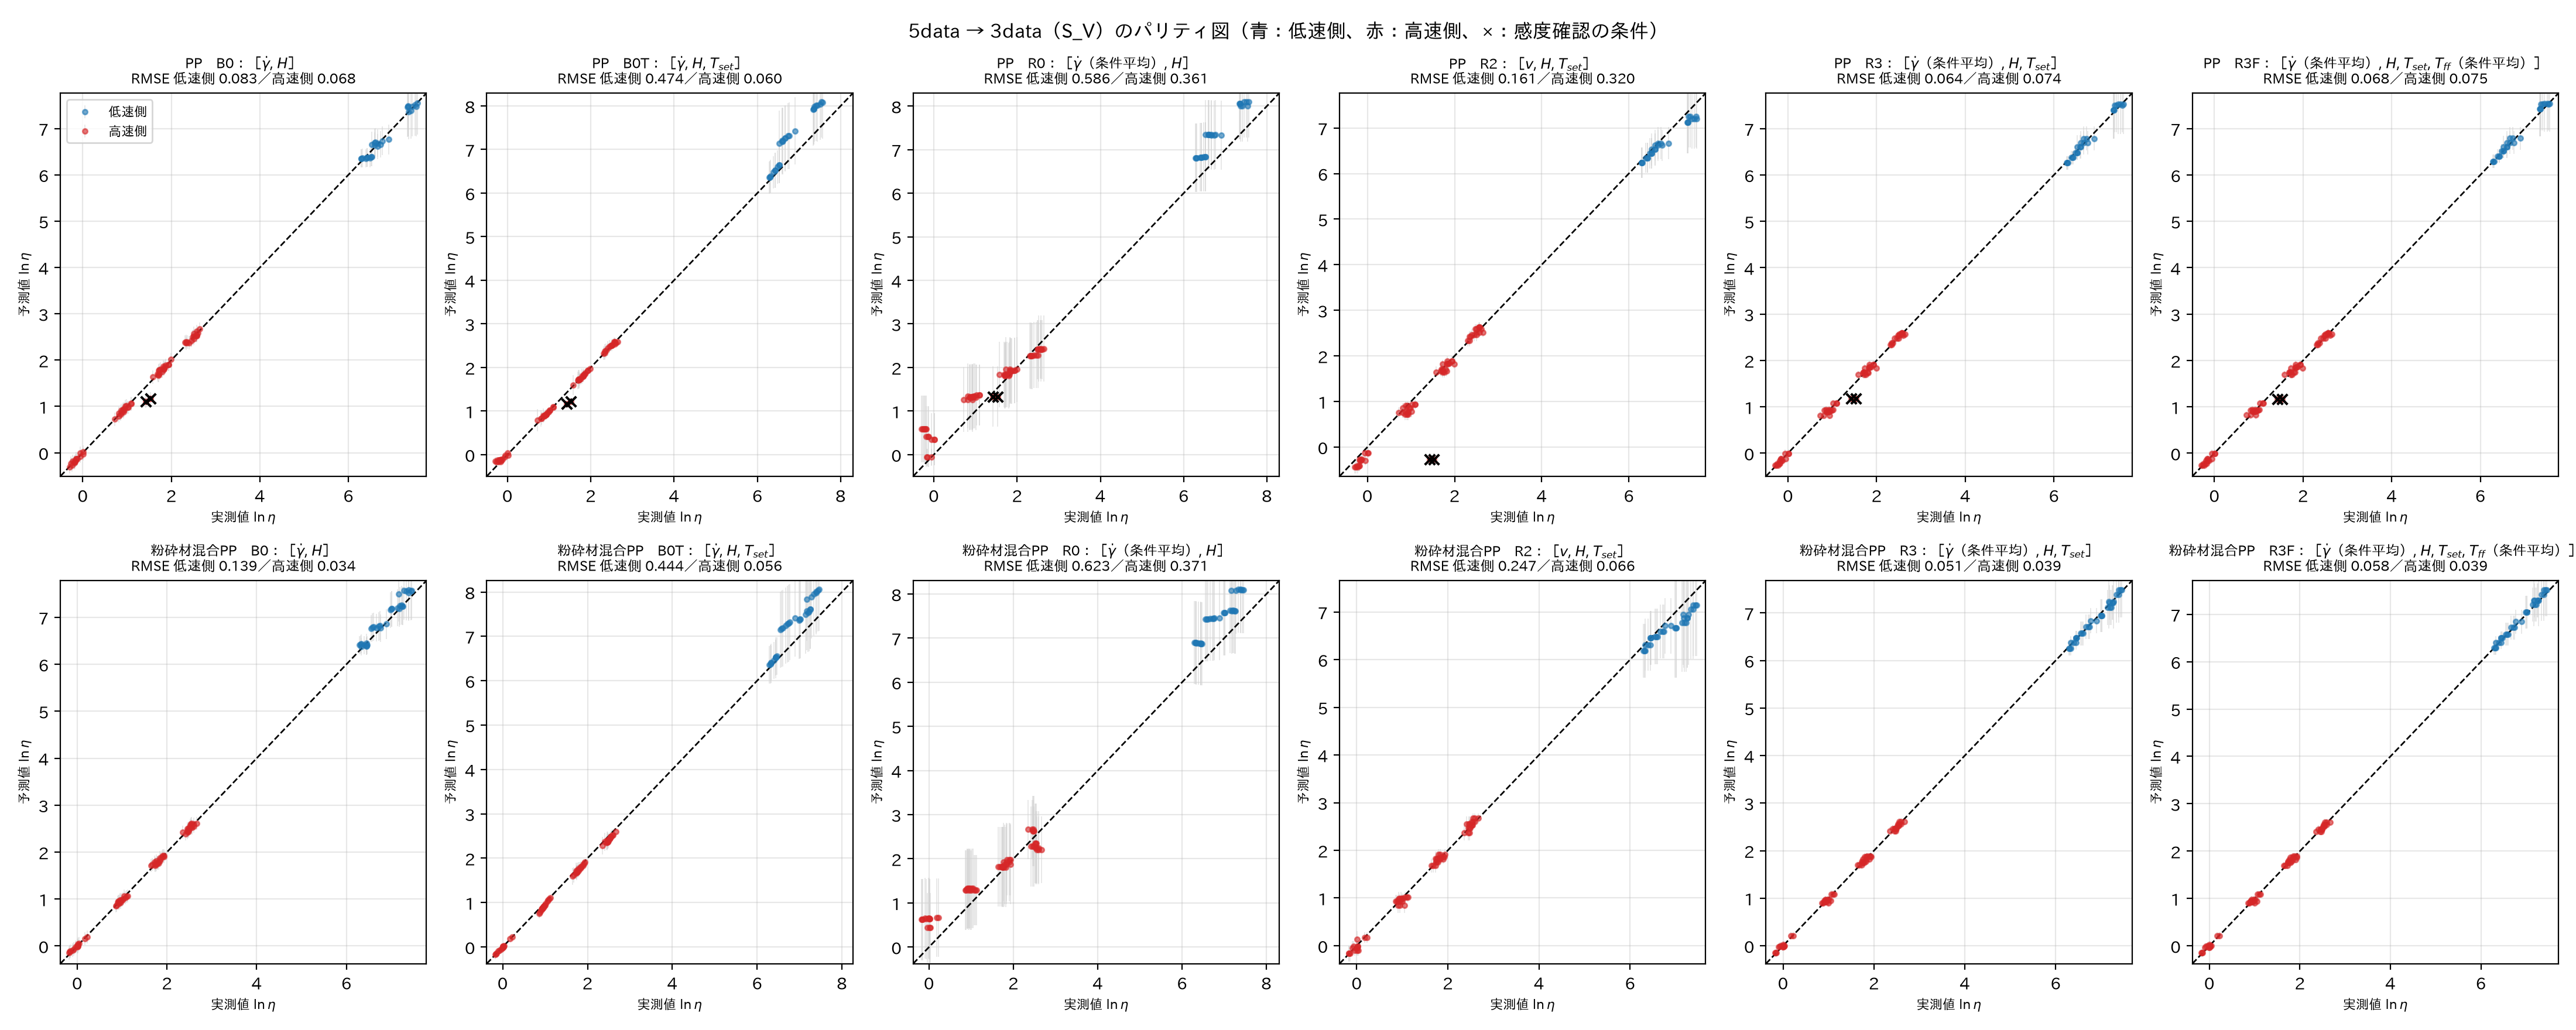
\includegraphics[width=\linewidth]{fig2_parity_S_V.png}
\caption{5data $\to$ 3data のパリティ図（上段 PP、下段 粉砕材混合 PP）}
\end{figure}
\begin{points}
\pt{ファイル}\file{results/step3b/fig2_parity_S_V.png}
\pt{何を示す図か}6つのモデル（列）の予測が、検証データでどれだけ当たったかを、2つの材料（行）で比べる図です。
\pt{軸と記号}横軸は実測の $\ln\eta$、縦軸は予測の $\ln\eta$。青が低速側、赤が高速側、灰色の縦線が 95\% 予測区間、黒い破線が理想線、黒い × が感度確認の条件（P03）です。各パネルの上に、モデルと低速側・高速側の RMSE を示しました。
\pt{見るポイント}点が破線に沿っているか。青い点（低速側）が破線から離れていないか。灰色の縦線が破線にかかっているか。
\pt{今回の結果}B0T（ショットごと）は、高速側（赤）は破線に乗りますが、低速側（青）は破線から下に外れます（RMSE：PP 0.474、粉砕材混合 PP 0.444）。R3（条件平均）は、低速側も破線に近く（RMSE：PP 0.064、粉砕材混合 PP 0.051）、高速側も当たります。温度を入れない R0 は、低速側（0.586）も高速側（0.361）も大きく外れます。B0（温度なし、ショットごと）は低速側も当たっているように見えますが（0.083）、これは、ショットごとの $\gd$ が、設定温度の情報を含んでしまっているためです（同じ射出速度でも、$\gd$ は温度で少し違う）。PP の高速側で、黒い × （P03：PP の 190 ℃・0.5 mm・320 mm/s）が破線から離れ、高速側の RMSE を押し上げます（R3：0.074 → P03 を除くと 0.053）。
\end{points}

% ---------------------------------------------------------------------
\subsection{図3：S\_T（210 ℃ のホールドアウト）のパリティ図}
\begin{figure}[H]
\centering
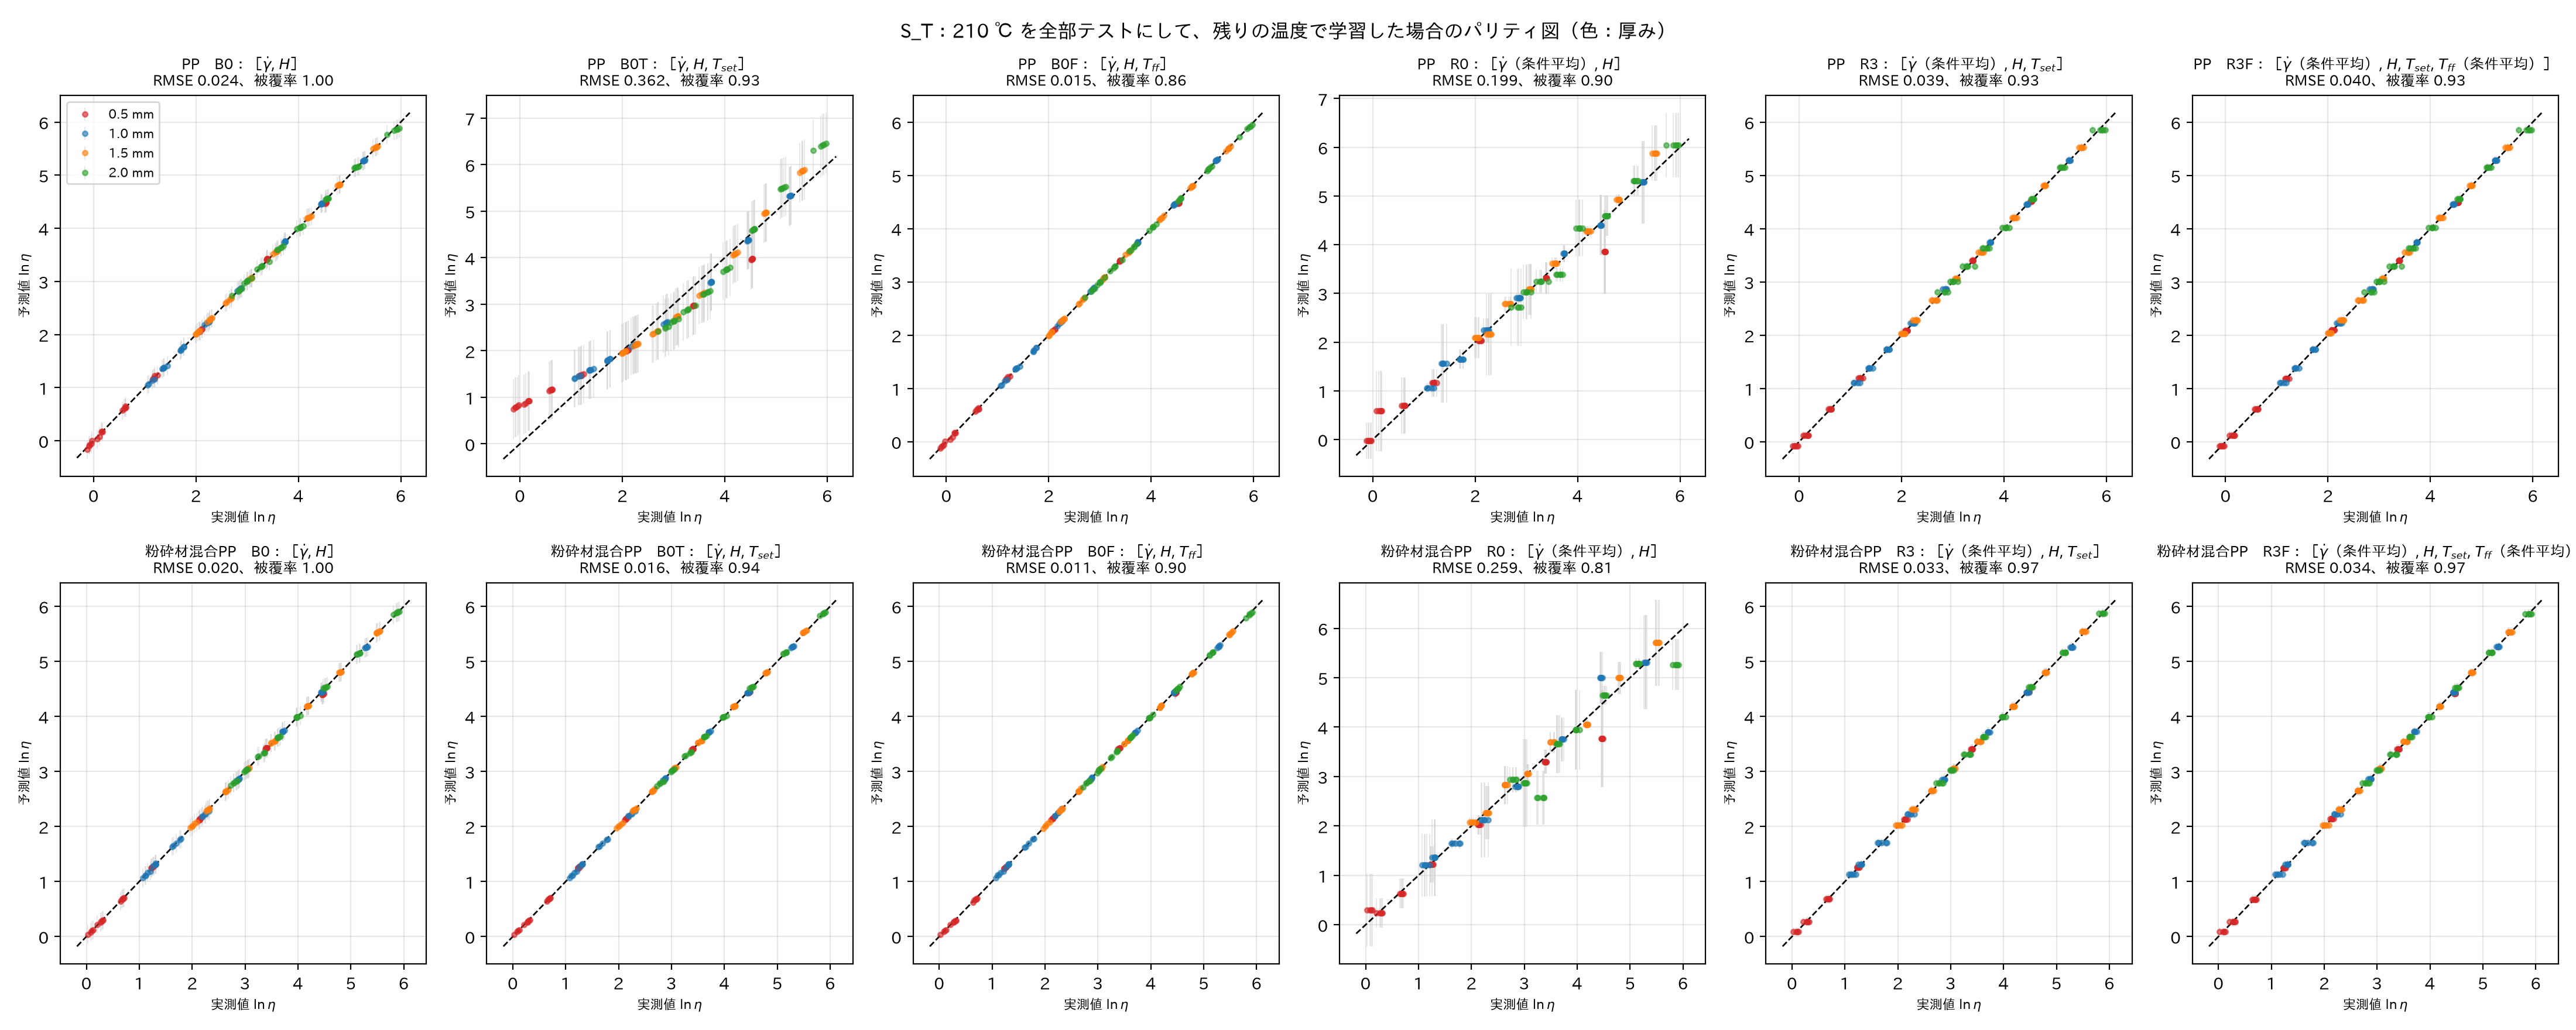
\includegraphics[width=\linewidth]{fig3_parity_S_T.png}
\caption{210 ℃ を全部テストにして、190・230 ℃ で学習した場合のパリティ図（色：厚み）}
\end{figure}
\begin{points}
\pt{ファイル}\file{results/step3b/fig3_parity_S_T.png}
\pt{何を示す図か}設定温度の内挿の検証です。190 ℃ と 230 ℃ のデータだけで学習し、間の 210 ℃ を予測します。
\pt{軸と記号}図2と同じです。色は厚み（赤 0.5 mm、青 1.0 mm、橙 1.5 mm、緑 2.0 mm）。
\pt{見るポイント}$\Tset$ を入力に持つモデル（B0T、R3、R3F）が、持たないモデル（B0、R0）より当たっているか。
\pt{今回の結果}PP の B0T（$\Tset$ あり、ショットごと）は、210 ℃ の予測が大きく外れます（RMSE 0.362）。このとき学習された $\Tset$ の長さスケールは 0.012（下限 0.01 に張り付き）で、「190 ℃ と 230 ℃ は別物」と見なす（間の 210 ℃ を補間できない）解になっていました。粉砕材混合 PP の B0T（0.016）や、R3（PP 0.039、粉砕材混合 PP 0.033）は、破線に乗ります。$\Tset$ を持たない R0 は、PP で 0.199、粉砕材混合 PP で 0.259 と、大きく外れ、温度の情報が必要なことが分かります。$\Tff$ を持つ B0F は、S\_T では当たります（PP 0.015）が、これは $\Tff$ が温度を反映しているためです。
\end{points}

% ---------------------------------------------------------------------
\subsection{図4：分け方ごとの評価の違い}
\begin{figure}[H]
\centering
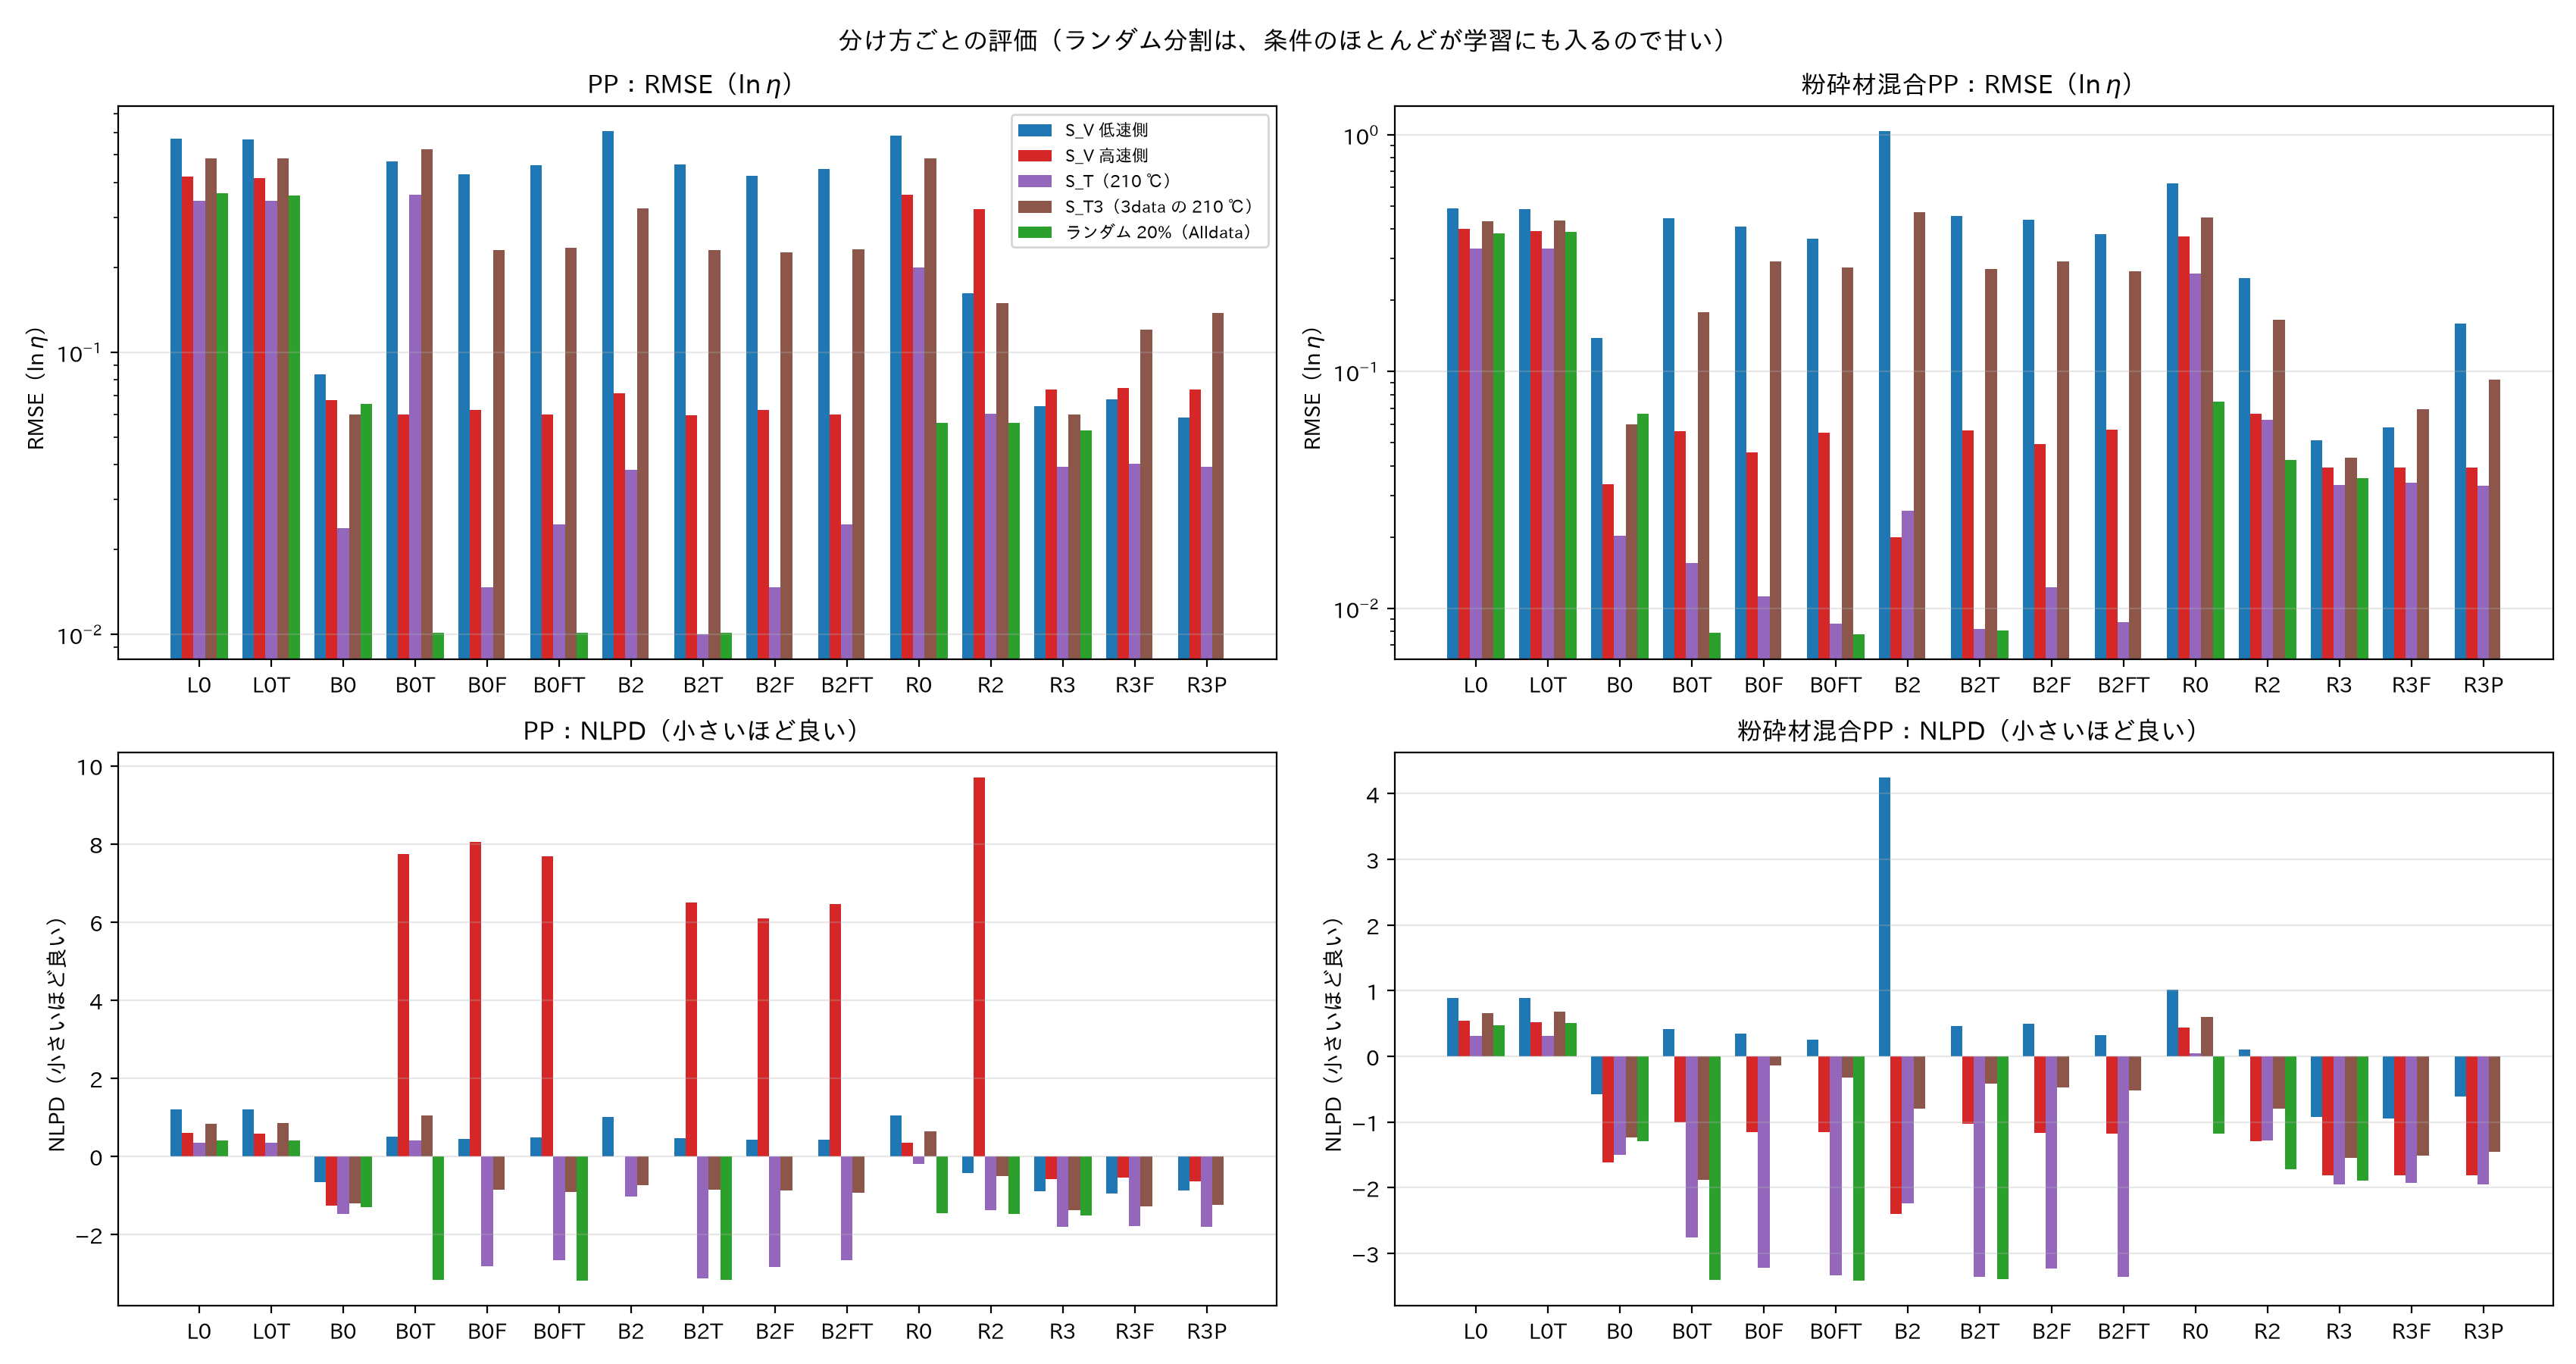
\includegraphics[width=\linewidth]{fig4_metrics_by_split.png}
\caption{分け方ごとの RMSE（上段）と NLPD（下段）}
\end{figure}
\begin{points}
\pt{ファイル}\file{results/step3b/fig4_metrics_by_split.png}
\pt{何を示す図か}15 のモデルを、5つの検証の方法で比べた図です。左が PP、右が粉砕材混合 PP。
\pt{軸と記号}横軸がモデル、縦軸が RMSE（上段。対数軸）と NLPD（下段。小さいほど良い）。棒の色が検証の方法（青 S\_V 低速側、赤 S\_V 高速側、紫 S\_T、茶 S\_T3、緑 ランダム 20\%）。ランダム 20\% を計算していないモデルは、棒が 0 です。
\pt{見るポイント}同じモデルで、緑の棒（ランダム）が、ほかの棒より大幅に低くないか（評価が甘い）。
\pt{今回の結果}B0T（ショットごと）は、ランダム 20\% の RMSE が 0.010（PP）と非常に小さい一方、S\_V の低速側は 0.474 で、約 47 倍も違います。ランダム分割は、同じ条件のショットが学習にも入るので、評価が甘くなります。R3 は、ランダム分割（0.053）と S\_V の低速側（0.064）の差が小さく、条件ごとの入力のため、「同じ条件を学習に入れてしまう」影響が小さい評価になっています。線形回帰（L0・L0T）は、どの検証でも大きく外れ、基準になりません（S\_V 低速側 0.567）。
\end{points}

% ---------------------------------------------------------------------
\subsection{図5：設定温度の効果}
\begin{figure}[H]
\centering
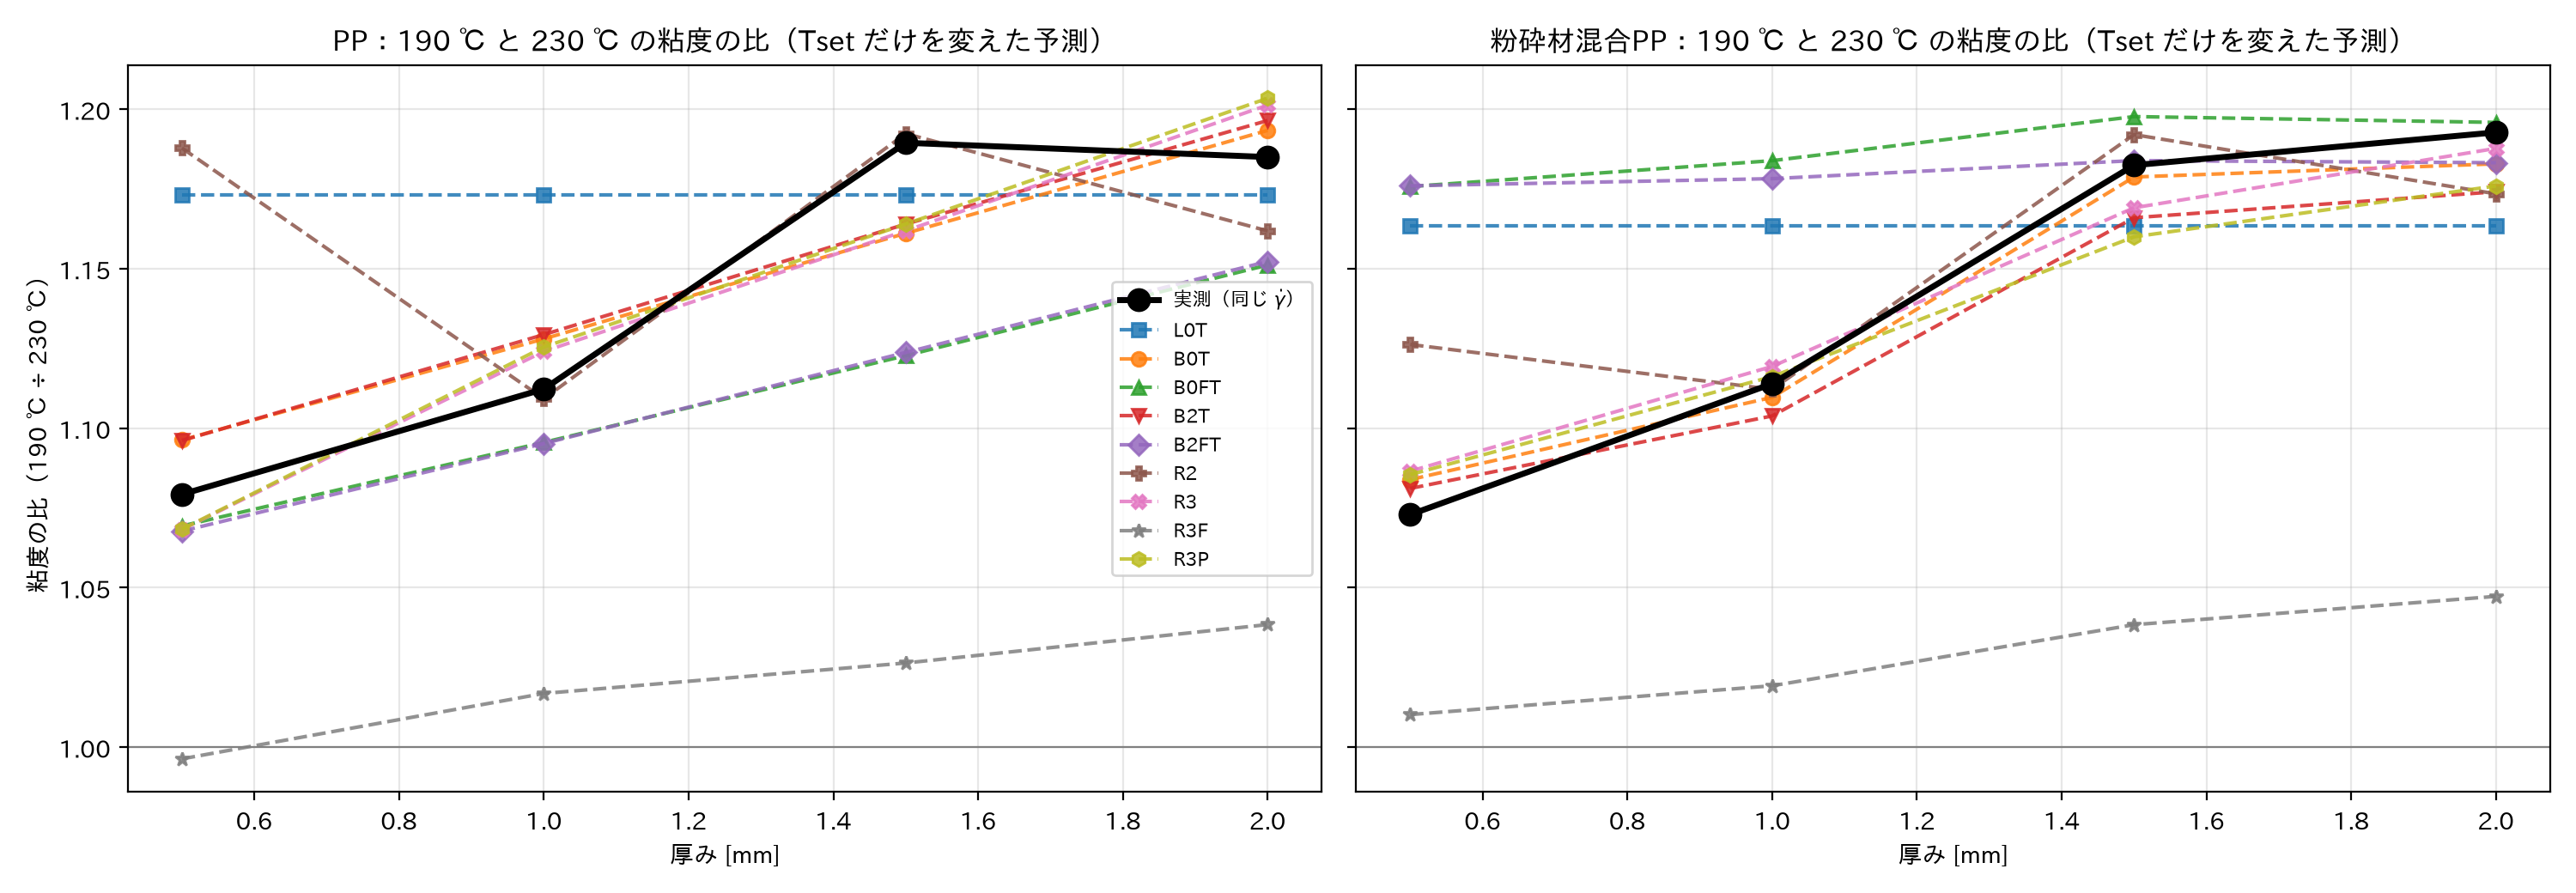
\includegraphics[width=\linewidth]{fig5_temperature_effect.png}
\caption{190 ℃ と 230 ℃ の粘度の比。黒の太線が実測}
\end{figure}
\begin{points}
\pt{ファイル}\file{results/step3b/fig5_temperature_effect.png}
\pt{何を示す図か}同じ厚み・同じせん断速度で、190 ℃ の粘度が 230 ℃ の何倍かを、実測とモデルの予測で比べた図です（モデルは、$\Tset$ だけを 190 ℃・230 ℃ にして予測）。
\pt{軸と記号}横軸が厚み、縦軸が粘度の比。黒の太線が実測、色の線がモデル（$\Tset$ を入力に持つモデルだけ）。
\pt{見るポイント}実測の線（厚いほど大きい）に、モデルの線が近いか。水平な線（厚みによらず一定）になっていないか。
\pt{今回の結果}実測の比は、PP で 1.08〜1.19、粉砕材混合 PP で 1.07〜1.19（厚いほど大きい）です。R3 の予測は、PP で 1.07〜1.20（実測との差の最大 0.028）、粉砕材混合 PP で 1.09〜1.19（同 0.014）で、実測の傾向（厚いほど大きい）まで再現します。B0T も近い値です（PP 1.10〜1.19）。線形回帰の L0T は、厚みによらず一定の比（約 1.17）で、厚み依存を表せません。R2（設定値だけ）は、厚みで上下に振れます。R3F（$\Tff$ あり）は、ほとんど 1 で、温度の効果を $\Tset$ では表せません。B0FT・B2FT（$\Tff$ あり、ショットごと）は、PP で比が小さくなります（1.07〜1.15）。
\end{points}

% ---------------------------------------------------------------------
\subsection{図6：ARD の感度}
\begin{figure}[H]
\centering
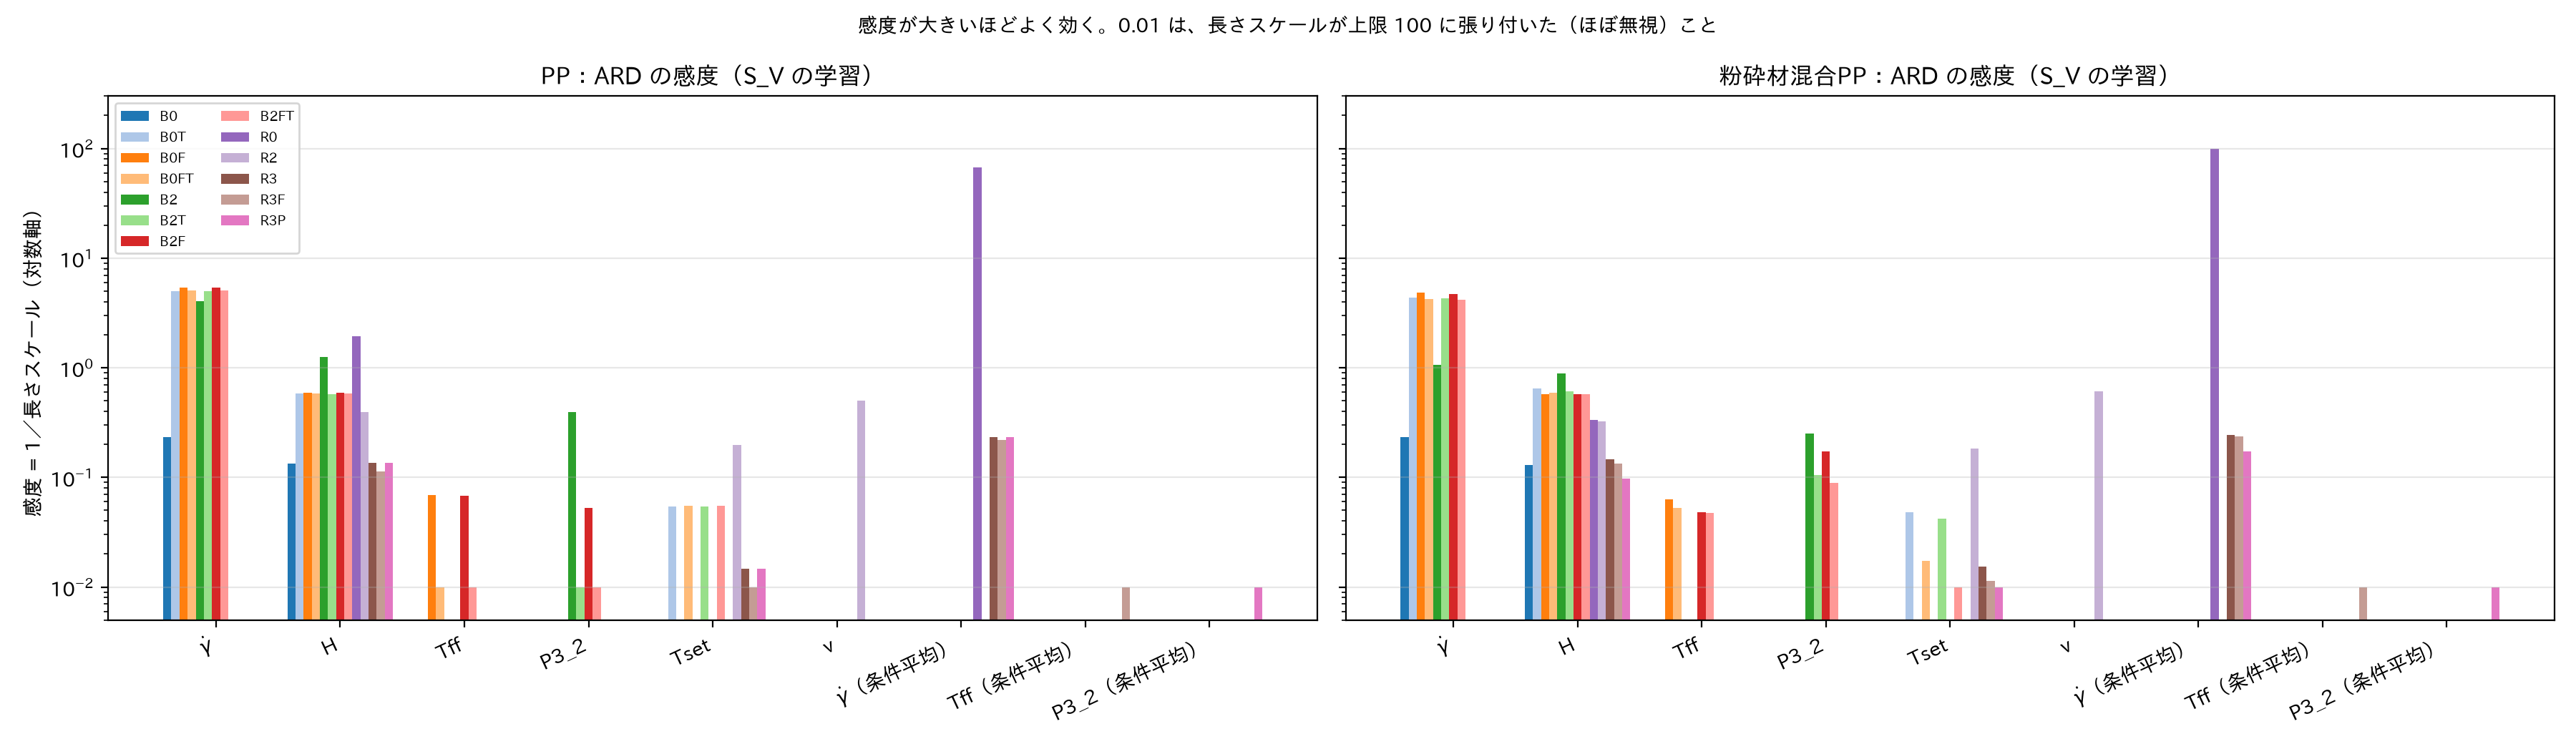
\includegraphics[width=\linewidth]{fig6_ard_sensitivity.png}
\caption{GPR の入力ごとの感度（1／長さスケール）}
\end{figure}
\begin{points}
\pt{ファイル}\file{results/step3b/fig6_ard_sensitivity.png}
\pt{何を示す図か}GPR が、どの入力をよく使っているかを示す図です（5data で学習したモデル）。
\pt{軸と記号}横軸が入力、縦軸が感度（長さスケールの逆数。標準化した入力に対する値。対数軸）。棒の色がモデル。棒がない入力は、そのモデルに入っていません。感度 0.01 は、長さスケールが上限の 100 に張り付いた（ほとんど使われていない）ことを表し、100 に近い値は、下限の 0.01 に近い（入力のわずかな違いに敏感）ことを表します。
\pt{見るポイント}$\Tset$ の棒が、モデルによってどれくらい違うか（0 に近いなら、ほとんど使われていない）。$\gd$ の棒が、B 系（ショットごと）と R 系（条件平均）で、どれだけ違うか。
\pt{今回の結果}B 系（ショットごと）では、$\gd$ の感度が大きく（長さスケール 0.20。標準化後）、$\Tset$ は 18 と小さな感度です。R 系（条件平均）では、$\gd$（条件平均）の長さスケールが 4.3 と大きく（なめらか）、$\Tset$ は 68 と、探索範囲の上限（100）に近い値です。これは、温度の効果が、Matern カーネルの部分ではなく、主に線形カーネルの部分で（直線的に）表されていることを意味します。R3F・R3P で足した $\Tff$・\PII\ の長さスケールは、上限（100）に張り付き、Matern の部分では使われていません。温度を入れない R0 は、$\gd$（条件平均）の長さスケールが 0.015（PP。下限 0.01 の近く）と極端に小さく、感度が最も大きく見えます。温度による粘度の違いを、$\gd$ のわずかな違いで説明しようとして、曲線をでこぼこにしているためです（図は対数軸）。
\end{points}

% ---------------------------------------------------------------------
\subsection{図7：ノイズの標準偏差と純粋誤差}
\begin{figure}[H]
\centering
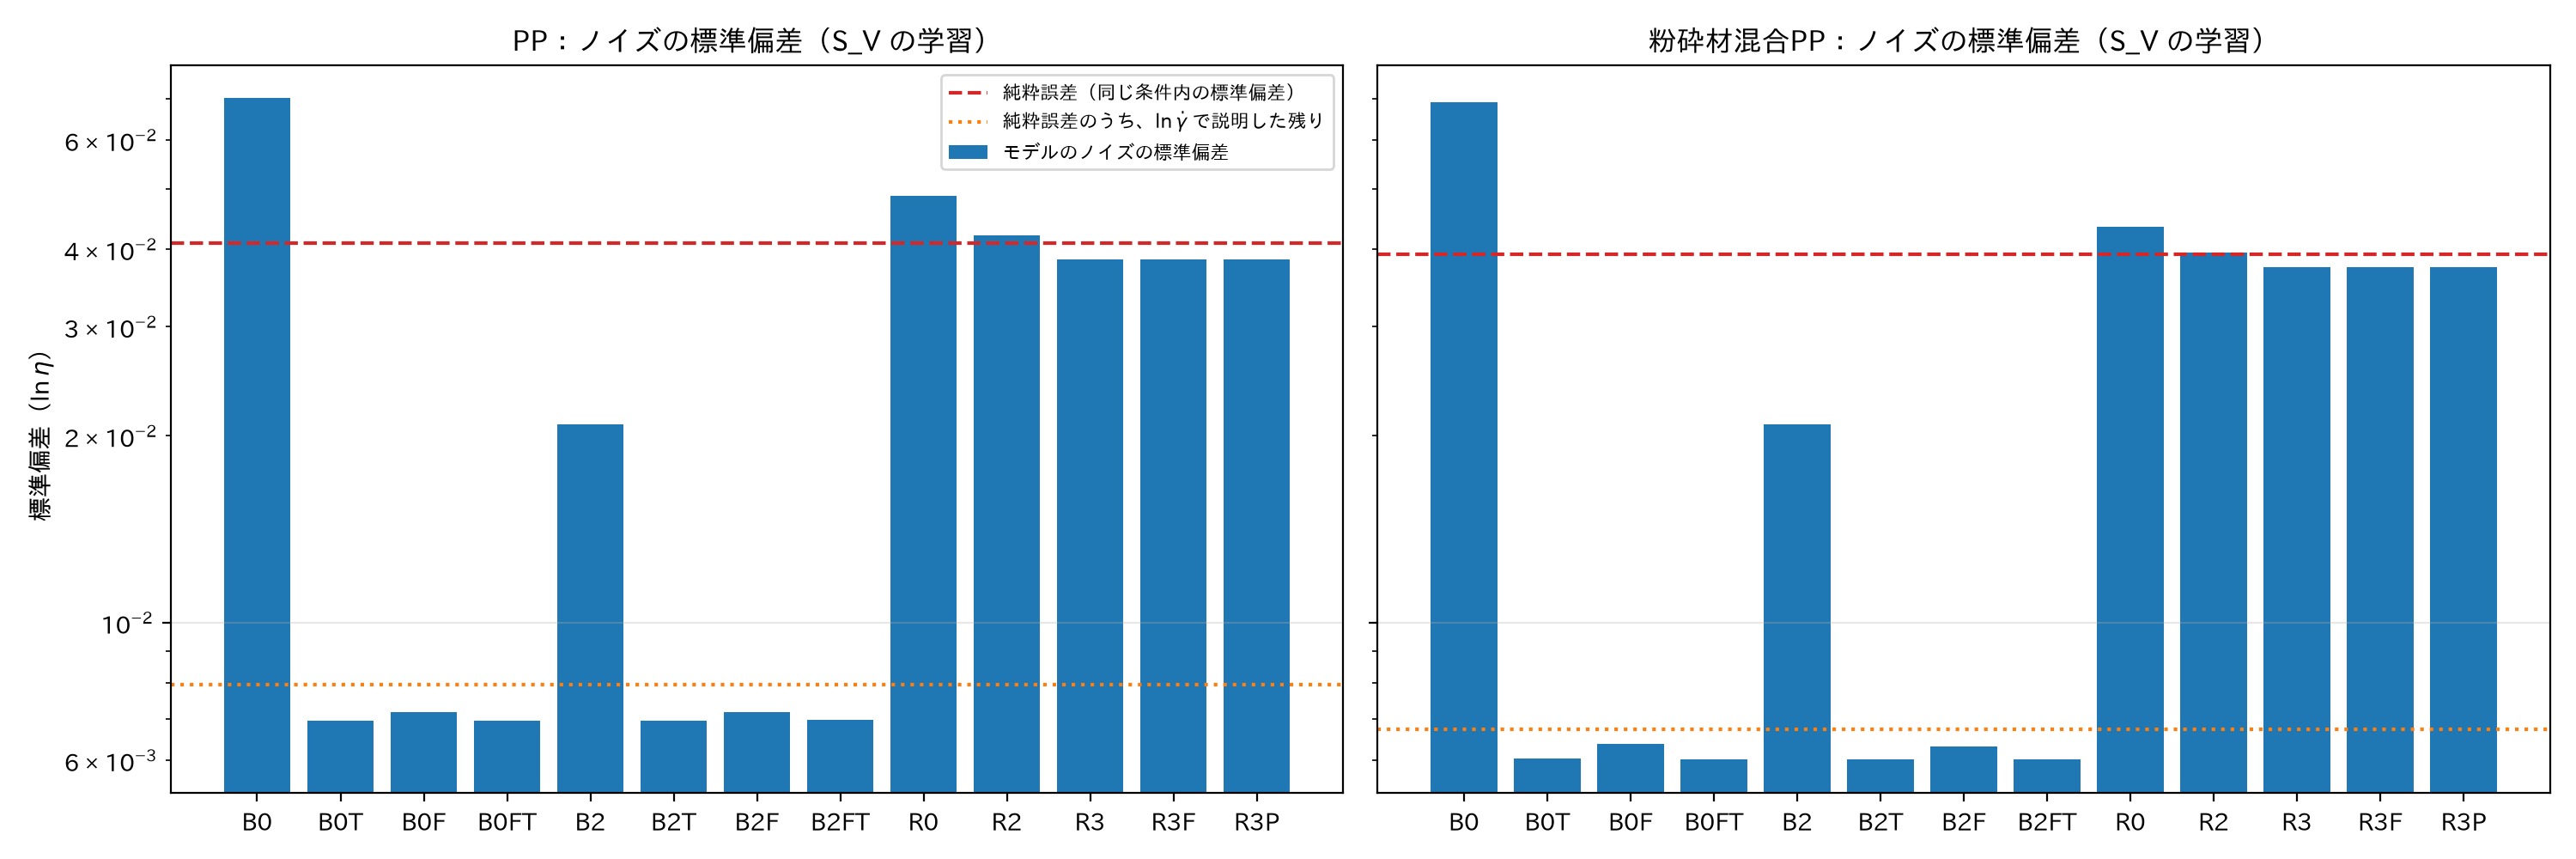
\includegraphics[width=\linewidth]{fig7_noise_vs_pure_error.png}
\caption{GPR のノイズの標準偏差と、同じ条件内のばらつき（純粋誤差）}
\end{figure}
\begin{points}
\pt{ファイル}\file{results/step3b/fig7_noise_vs_pure_error.png}
\pt{何を示す図か}GPR が見積もる「ノイズ」（ショット間のばらつき）の大きさと、実際の同じ条件内のばらつき（純粋誤差）を比べる図です。
\pt{軸と記号}横軸がモデル、縦軸が $\ln\eta$ の標準偏差（対数軸）。青い棒がモデルのノイズの標準偏差、赤い破線が純粋誤差、橙の点線が、純粋誤差のうち $\ln\gd$ で説明できなかった残りです。
\pt{見るポイント}青い棒が、赤い破線に近いか（成形条件から見たばらつきを表している）、橙の点線に近いか（ショットごとの $\gd$ で説明できる分を引いた残りしか表していない）。
\pt{今回の結果}B 系（B0T など）のノイズの標準偏差は 0.0069（PP）と、純粋誤差（0.0409）よりずっと小さく、「$\ln\gd$ で説明した残り」（0.0079）に近い値です。ショットごとの $\gd$ を入れると、同じ条件内のばらつきの大部分が説明されるためです。R 系（R3 など）のノイズの標準偏差は 0.0385（PP）・0.0374（粉砕材混合 PP）で、純粋誤差（0.0409・0.0393）に近く、成形条件から見たばらつきを表しています。B0（温度なし）のノイズ（0.0700）が大きいのは、温度の違いを、ノイズとして吸収しているためです。
\end{points}

% ---------------------------------------------------------------------
\subsection{高解像度のグラフ（報告書・発表資料用）}
\begin{points}
\pt{ファイル}\file{results/step3b/highres/hr_<材料>_<モデル>_<学習>_by-thickness_<厚み>mm.png}（厚みごとに 1 枚。3 つの設定温度の曲線）と、\file{..._by-temperature_<温度>C.png}（設定温度ごとに 1 枚。4 つの厚みの曲線）。Git には入れません（ノートのセルで、いつでも作り直せます）。
\pt{何を示す図か}GPR6月のノートのセル9-2 と同じ見せ方の、せん断速度 ― 粘度の学習結果グラフです。\textbf{600 dpi（15 $\times$ 10 インチ）}で、1 枚に 1 つのグラフを保存します。線は予測の平均、帯は 95\% 予測区間、塗りつぶしの点は学習に使った条件（条件平均）、白抜きの点は学習に使わなかった条件（検証）、黒い $\times$ は問題データ一覧の「感度確認」の条件です。既定は、R3（5data で学習）を、PP と粉砕材混合 PP について描きます。
\pt{変え方}ノート11章の「高解像度のグラフ」のセルの先頭に、設定エリアがあります（描くモデル・材料・学習の種類、レイアウト、帯、点、軸の範囲、予測線の延長、図の大きさ・解像度、文字・点・線の大きさ、タイトルと軸名の表示、保存形式 png・pdf・svg）。\textbf{そのセルの設定だけを直して、そのセルだけを実行し直せます}（学習はやり直しません。ノート全体を一度実行した後で）。
\pt{見るポイント}(1) 設定温度ごとの線が、温度の順に並ぶか。(2) 白抜きの点（外挿の検証データ）が、線と帯の上に乗るか。(3) 帯が、学習範囲の外で広がるか。
\end{points}

% =====================================================================
\section{表の見方}

\begin{table}[H]
\caption{検証データ（5data $\to$ 3data）での指標：PP（$\ln\eta$。\file{metrics.csv}）。高速側の括弧内は、P03 を評価から除いた値}\label{tab:sv_pp}
\begin{tabularx}{\linewidth}{@{}l*{7}{r}@{}}
\toprule
 & \multicolumn{3}{c}{RMSE} & \multicolumn{2}{c}{被覆率} & \multicolumn{2}{c}{NLPD} \\
\cmidrule(lr){2-4}\cmidrule(lr){5-6}\cmidrule(l){7-8}
モデル & 低速側 & 高速側 & （P03 除く） & 低速側 & 高速側 & 低速側 & 高速側 \\
\midrule
L0 & 0.570 & 0.420 & 0.425 & 0.74 & 0.81 & 1.20 & 0.59 \\
L0T & 0.567 & 0.413 & 0.419 & 0.89 & 0.79 & 1.21 & 0.58 \\
B0 & 0.083 & 0.068 & 0.034 & 1.00 & 0.97 & $-0.67$ & $-1.26$ \\
B0T & 0.474 & 0.060 & 0.035 & 1.00 & 0.78 & 0.50 & 7.74 \\
B0F & 0.426 & 0.062 & 0.038 & 1.00 & 0.78 & 0.44 & 8.04 \\
B0FT & 0.460 & 0.060 & 0.036 & 1.00 & 0.78 & 0.47 & 7.68 \\
B2 & 0.607 & 0.072 & 0.035 & 1.00 & 0.93 & 1.01 & $-0.01$ \\
B2T & 0.462 & 0.060 & 0.035 & 1.00 & 0.78 & 0.45 & 6.50 \\
B2F & 0.421 & 0.062 & 0.038 & 1.00 & 0.78 & 0.43 & 6.09 \\
B2FT & 0.447 & 0.060 & 0.036 & 1.00 & 0.78 & 0.43 & 6.46 \\
R0 & 0.586 & 0.361 & 0.365 & 0.96 & 0.91 & 1.05 & 0.35 \\
R2 & 0.161 & 0.320 & 0.117 & 1.00 & 0.59 & $-0.43$ & 9.70 \\
R3 & 0.064 & 0.074 & 0.053 & 1.00 & 0.85 & $-0.90$ & $-0.59$ \\
R3F & 0.068 & 0.075 & 0.053 & 1.00 & 0.85 & $-0.96$ & $-0.55$ \\
R3P & 0.059 & 0.074 & 0.053 & 1.00 & 0.85 & $-0.88$ & $-0.64$ \\
\bottomrule
\end{tabularx}
\end{table}

\begin{table}[H]
\caption{検証データ（5data $\to$ 3data）での指標：粉砕材混合 PP}\label{tab:sv_mix}
\begin{tabularx}{\linewidth}{@{}l*{7}{r}@{}}
\toprule
 & \multicolumn{3}{c}{RMSE} & \multicolumn{2}{c}{被覆率} & \multicolumn{2}{c}{NLPD} \\
\cmidrule(lr){2-4}\cmidrule(lr){5-6}\cmidrule(l){7-8}
モデル & 低速側 & 高速側 & （P03 除く） & 低速側 & 高速側 & 低速側 & 高速側 \\
\midrule
L0 & 0.490 & 0.400 & --- & 0.85 & 0.81 & 0.89 & 0.54 \\
L0T & 0.486 & 0.392 & --- & 0.91 & 0.81 & 0.89 & 0.52 \\
B0 & 0.139 & 0.034 & --- & 1.00 & 1.00 & $-0.58$ & $-1.61$ \\
B0T & 0.444 & 0.056 & --- & 1.00 & 0.75 & 0.41 & $-1.00$ \\
B0F & 0.411 & 0.046 & --- & 1.00 & 0.79 & 0.34 & $-1.16$ \\
B0FT & 0.365 & 0.055 & --- & 1.00 & 0.78 & 0.25 & $-1.15$ \\
B2 & 1.035 & 0.020 & --- & 0.00 & 1.00 & 4.24 & $-2.41$ \\
B2T & 0.454 & 0.056 & --- & 1.00 & 0.78 & 0.46 & $-1.03$ \\
B2F & 0.437 & 0.050 & --- & 1.00 & 0.76 & 0.50 & $-1.17$ \\
B2FT & 0.380 & 0.057 & --- & 1.00 & 0.78 & 0.32 & $-1.17$ \\
R0 & 0.623 & 0.371 & --- & 1.00 & 1.00 & 1.01 & 0.44 \\
R2 & 0.247 & 0.066 & --- & 1.00 & 0.93 & 0.11 & $-1.30$ \\
R3 & 0.051 & 0.039 & --- & 1.00 & 0.96 & $-0.92$ & $-1.82$ \\
R3F & 0.058 & 0.039 & --- & 1.00 & 0.96 & $-0.95$ & $-1.82$ \\
R3P & 0.159 & 0.039 & --- & 1.00 & 0.96 & $-0.61$ & $-1.82$ \\
\bottomrule
\end{tabularx}
\end{table}

\begin{table}[H]
\caption{S\_T（5data の 210 ℃）と S\_T3（3data の 210 ℃）での指標（\file{metrics.csv}）。RMSE／NLPD}\label{tab:st}
\begin{tabularx}{\linewidth}{@{}l*{4}{r}@{}}
\toprule
 & \multicolumn{2}{c}{PP} & \multicolumn{2}{c}{粉砕材混合 PP} \\
\cmidrule(lr){2-3}\cmidrule(l){4-5}
モデル & S\_T & S\_T3 & S\_T & S\_T3 \\
\midrule
L0 & 0.343／0.35 & 0.486／0.83 & 0.331／0.31 & 0.433／0.66 \\
L0T & 0.343／0.35 & 0.487／0.86 & 0.331／0.31 & 0.433／0.68 \\
B0 & 0.024／$-1.48$ & 0.060／$-1.21$ & 0.020／$-1.50$ & 0.060／$-1.23$ \\
B0T & 0.362／0.41 & 0.523／1.05 & 0.016／$-2.76$ & 0.178／$-1.88$ \\
B0F & 0.015／$-2.82$ & 0.231／$-0.86$ & 0.011／$-3.22$ & 0.293／$-0.14$ \\
B0FT & 0.025／$-2.65$ & 0.234／$-0.92$ & 0.009／$-3.34$ & 0.275／$-0.32$ \\
B2 & 0.038／$-1.03$ & 0.323／$-0.74$ & 0.026／$-2.24$ & 0.471／$-0.80$ \\
B2T & 0.010／$-3.13$ & 0.230／$-0.86$ & 0.008／$-3.36$ & 0.272／$-0.42$ \\
B2F & 0.015／$-2.83$ & 0.226／$-0.87$ & 0.012／$-3.24$ & 0.292／$-0.47$ \\
B2FT & 0.024／$-2.66$ & 0.232／$-0.93$ & 0.009／$-3.36$ & 0.265／$-0.52$ \\
R0 & 0.199／$-0.19$ & 0.486／0.65 & 0.259／0.05 & 0.446／0.60 \\
R2 & 0.060／$-1.39$ & 0.149／$-0.50$ & 0.063／$-1.28$ & 0.166／$-0.79$ \\
R3 & 0.039／$-1.82$ & 0.060／$-1.38$ & 0.033／$-1.95$ & 0.043／$-1.55$ \\
R3F & 0.040／$-1.79$ & 0.120／$-1.29$ & 0.034／$-1.93$ & 0.069／$-1.51$ \\
R3P & 0.039／$-1.82$ & 0.138／$-1.25$ & 0.033／$-1.95$ & 0.092／$-1.46$ \\
\bottomrule
\end{tabularx}
\end{table}

\begin{table}[H]
\caption{190 ℃ と 230 ℃ の粘度の比（S\_V の学習。\file{tset_effect.csv}、\file{observed_ratio.csv}）}\label{tab:eff}
\begin{tabularx}{\linewidth}{@{}l>{\raggedright\arraybackslash}p{5\zw}rrrr@{}}
\toprule
材料 & モデル & 0.5 mm & 1.0 mm & 1.5 mm & 2.0 mm \\
\midrule
PP & 実測 & 1.079 & 1.112 & 1.189 & 1.185 \\
 & L0T & 1.173 & 1.173 & 1.173 & 1.173 \\
 & B0T & 1.096 & 1.128 & 1.161 & 1.193 \\
 & B0FT & 1.069 & 1.096 & 1.123 & 1.151 \\
 & B2T & 1.096 & 1.129 & 1.164 & 1.196 \\
 & B2FT & 1.068 & 1.095 & 1.124 & 1.152 \\
 & R2 & 1.188 & 1.109 & 1.192 & 1.162 \\
 & R3 & 1.068 & 1.124 & 1.162 & 1.201 \\
 & R3F & 0.996 & 1.017 & 1.026 & 1.038 \\
 & R3P & 1.068 & 1.125 & 1.164 & 1.203 \\
粉砕材混合 PP & 実測 & 1.073 & 1.114 & 1.182 & 1.193 \\
 & L0T & 1.163 & 1.163 & 1.163 & 1.163 \\
 & B0T & 1.084 & 1.110 & 1.179 & 1.183 \\
 & B0FT & 1.176 & 1.184 & 1.198 & 1.196 \\
 & B2T & 1.081 & 1.104 & 1.166 & 1.174 \\
 & B2FT & 1.176 & 1.178 & 1.184 & 1.183 \\
 & R2 & 1.126 & 1.112 & 1.192 & 1.173 \\
 & R3 & 1.087 & 1.119 & 1.169 & 1.188 \\
 & R3F & 1.010 & 1.019 & 1.038 & 1.047 \\
 & R3P & 1.085 & 1.116 & 1.160 & 1.176 \\
\bottomrule
\end{tabularx}
\end{table}

\begin{table}[H]
\caption{ノイズの標準偏差と純粋誤差（S\_V の学習。$\ln\eta$。\file{kernels.csv}）。「張り付き」：長さスケールが探索範囲の端（S\_V・S\_T のどちらか）}\label{tab:noise}
\begin{tabularx}{\linewidth}{@{}l>{\raggedright\arraybackslash}p{4\zw}rrrl@{}}
\toprule
材料 & モデル & ノイズの標準偏差 & 純粋誤差 & 純粋誤差の残り & 張り付き \\
\midrule
PP & B0 & 0.0700 & 0.0409 & 0.0079 & --- \\
 & B0T & 0.0069 & 0.0409 & 0.0079 & --- \\
 & B0F & 0.0072 & 0.0409 & 0.0079 & --- \\
 & B0FT & 0.0070 & 0.0409 & 0.0079 & S\_V、S\_T \\
 & B2 & 0.0209 & 0.0409 & 0.0079 & --- \\
 & B2T & 0.0070 & 0.0409 & 0.0079 & S\_V \\
 & B2F & 0.0072 & 0.0409 & 0.0079 & S\_T \\
 & B2FT & 0.0070 & 0.0409 & 0.0079 & S\_V、S\_T \\
 & R0 & 0.0488 & 0.0409 & 0.0079 & S\_T \\
 & R2 & 0.0420 & 0.0409 & 0.0079 & --- \\
 & R3 & 0.0385 & 0.0409 & 0.0079 & --- \\
 & R3F & 0.0385 & 0.0409 & 0.0079 & S\_V、S\_T \\
 & R3P & 0.0385 & 0.0409 & 0.0079 & S\_V、S\_T \\
粉砕材混合 PP & B0 & 0.0690 & 0.0393 & 0.0067 & --- \\
 & B0T & 0.0060 & 0.0393 & 0.0067 & --- \\
 & B0F & 0.0064 & 0.0393 & 0.0067 & S\_T \\
 & B0FT & 0.0060 & 0.0393 & 0.0067 & S\_T \\
 & B2 & 0.0209 & 0.0393 & 0.0067 & --- \\
 & B2T & 0.0060 & 0.0393 & 0.0067 & --- \\
 & B2F & 0.0063 & 0.0393 & 0.0067 & --- \\
 & B2FT & 0.0060 & 0.0393 & 0.0067 & S\_V、S\_T \\
 & R0 & 0.0435 & 0.0393 & 0.0067 & S\_V、S\_T \\
 & R2 & 0.0395 & 0.0393 & 0.0067 & --- \\
 & R3 & 0.0374 & 0.0393 & 0.0067 & --- \\
 & R3F & 0.0374 & 0.0393 & 0.0067 & S\_V、S\_T \\
 & R3P & 0.0374 & 0.0393 & 0.0067 & S\_V、S\_T \\
\bottomrule
\end{tabularx}
\end{table}

\begin{table}[H]
\caption{感度確認（学習から P02・P03 を除く。\file{sensitivity_judgement.csv}）。RMSE の変化が 10\% 以上かつ 0.01 以上のものを「大」}\label{tab:sens}
\begin{tabularx}{\linewidth}{@{}l>{\raggedright\arraybackslash}p{3\zw}>{\raggedright\arraybackslash}p{15\zw}rrrl@{}}
\toprule
材料 & モデル & 範囲 & すべて & 除く & 変化 [\%] & 影響 \\
\midrule
PP & B0T & S\_V 低速側 & 0.474 & 0.465 & $-2$ & 小 \\
PP & B0T & S\_V 高速側 & 0.060 & 0.060 & 0 & 小 \\
PP & B0T & S\_T & 0.362 & 0.010 & $-97$ & 大 \\
PP & B0T & S\_T3 & 0.523 & 0.229 & $-56$ & 大 \\
PP & B0T & S\_V 高速側（検証の P03 を評価から除く） & 0.060 & 0.035 & $-41$ & 大 \\
PP & R3 & S\_V 低速側 & 0.064 & 0.062 & $-3$ & 小 \\
PP & R3 & S\_V 高速側 & 0.074 & 0.074 & 0 & 小 \\
PP & R3 & S\_T & 0.039 & 0.039 & 0 & 小 \\
PP & R3 & S\_T3 & 0.060 & 0.063 & 4 & 小 \\
PP & R3 & S\_V 高速側（検証の P03 を評価から除く） & 0.074 & 0.053 & $-29$ & 大 \\
粉砕材混合 PP & B0T & S\_V 低速側 & 0.444 & 0.438 & $-1$ & 小 \\
粉砕材混合 PP & B0T & S\_V 高速側 & 0.056 & 0.055 & $-2$ & 小 \\
粉砕材混合 PP & B0T & S\_T & 0.016 & 0.015 & $-5$ & 小 \\
粉砕材混合 PP & B0T & S\_T3 & 0.178 & 0.152 & $-15$ & 大 \\
粉砕材混合 PP & B0T & S\_V 高速側（検証の P03 を評価から除く） & 0.056 & --- & --- & 小 \\
粉砕材混合 PP & R3 & S\_V 低速側 & 0.051 & 0.052 & 1 & 小 \\
粉砕材混合 PP & R3 & S\_V 高速側 & 0.039 & 0.039 & 0 & 小 \\
粉砕材混合 PP & R3 & S\_T & 0.033 & 0.033 & 0 & 小 \\
粉砕材混合 PP & R3 & S\_T3 & 0.043 & 0.044 & 2 & 小 \\
粉砕材混合 PP & R3 & S\_V 高速側（検証の P03 を評価から除く） & 0.039 & --- & --- & 小 \\
\bottomrule
\end{tabularx}
\end{table}

\begin{table}[H]
\caption{ランダム 20\%（従来の評価。RMSE。\file{metrics.csv}）と LOCO（\file{loco_metrics.csv}）}\label{tab:random}
\begin{tabularx}{\linewidth}{@{}l*{5}{r}@{}}
\toprule
 & \multicolumn{2}{c}{ランダム 20\%（PP）} & ランダム（混合） & \multicolumn{2}{c}{LOCO} \\
\cmidrule(lr){2-3}\cmidrule(lr){4-4}\cmidrule(l){5-6}
モデル & S\_R1 & S\_R2 & S\_R1 & PP & 混合 PP \\
\midrule
L0 & 0.366 & 0.389 & 0.383 & 0.374 & 0.354 \\
L0T & 0.360 & 0.391 & 0.389 & 0.371 & 0.351 \\
B0 & 0.066 & 0.071 & 0.066 & 0.084 & 0.081 \\
B0T & 0.010 & 0.009 & 0.008 & 0.044 & 0.016 \\
B0FT & 0.010 & 0.010 & 0.008 & 0.044 & 0.015 \\
B2T & 0.010 & 0.009 & 0.008 & 0.034 & 0.016 \\
R0 & 0.056 & 0.081 & 0.075 & 0.155 & 0.119 \\
R2 & 0.056 & 0.053 & 0.042 & 0.142 & 0.069 \\
R3 & 0.053 & 0.039 & 0.036 & 0.046 & 0.038 \\
B0F & --- & --- & --- & 0.044 & 0.019 \\
R3F & --- & --- & --- & 0.046 & 0.038 \\
R3P & --- & --- & --- & 0.046 & 0.038 \\
\bottomrule
\end{tabularx}
\end{table}

\begin{table}[H]
\caption{\file{results/step3b/} の表}
\begin{tabularx}{\linewidth}{@{}>{\raggedright\arraybackslash}p{19\zw}X@{}}
\toprule
ファイル & 中身と主な列 \\
\midrule
\file{metrics.csv} & 分け方・データ・モデル・評価の範囲ごとの指標。\file{split}（S\_V，S\_T，S\_T3，S\_R1，S\_R2、末尾の「\_感度除く」は、学習から感度確認の条件を除いたもの）、\file{data}（外れ値の なし・あり）、\file{subset}（全体・低速側・高速側、末尾の「（感度確認の条件を除く）」は P03 を評価から除いたもの）、\file{RMSE}、\file{R2}、\file{coverage95}、\file{NLPD}、\file{mean_sd}、\file{noise_sd}。 \\
\file{kernels.csv} & GPR のハイパーパラメータ。\file{amplitude}、\file{lin_amplitude}・\file{lin_sigma0}（線形項）、\file{ls_*}（長さスケール）、\file{noise_sd}、\file{pure_sd_ln_eta}（純粋誤差）、\file{LML}、\file{ls_at_bound}（長さスケールの張り付き）。 \\
\file{ols_coefficients.csv} & 線形回帰（L0，L0T）の係数。 \\
\file{loco_metrics.csv} & 条件を1つずつ抜く交差検証の指標。 \\
\file{tset_effect.csv} & 設定温度の効果（Tset だけを 190 → 230 ℃ にした予測の粘度比）。 \\
\file{observed_ratio.csv} & 設定温度の効果の実測（同じ $\gd$ での 190/230 ℃ の粘度比）。 \\
\file{sensitivity_judgement.csv} & 感度確認の結果（学習から除く前後の RMSE、予測比）。 \\
\bottomrule
\end{tabularx}
\end{table}

% =====================================================================
\section{結果のまとめ}

\subsection{観点ごとの結論}
\begin{enumerate}[itemsep=0.6ex,topsep=0.6ex]
\item \textbf{設定温度は要る}：条件平均の形（R 系）で、$\Tset$ を足すと（R0 $\to$ R3）、S\_T（210 ℃）の RMSE が PP で 0.199 から 0.039、粉砕材混合 PP で 0.259 から 0.033 に下がり、S\_V の低速側も 0.586 から 0.064（PP）に下がります（図2・図3、表\ref{tab:sv_pp}・\ref{tab:st}）。R3 は、190 ℃ と 230 ℃ の粘度の比も、実測に近く（PP 1.07〜1.20、実測 1.08〜1.19。実測との差の最大 0.028）、厚いほど大きいという厚み依存まで再現します（図5）。
\item \textbf{$\Tff$ は要らない（入れると有害）}：R3 に $\Tff$ を足しても（R3F）、S\_T の RMSE は変わらず（PP 0.039 $\to$ 0.040）、S\_T3 では悪くなります（0.060 $\to$ 0.120）。それだけでなく、$\Tff$ が温度の情報を持っているため、$\Tset$ だけを変えても予測が変わらなくなります（粘度比 1.00〜1.04。図1・図5）。$\Tff$ は、流動の結果として決まる値で、予測のときに事前に分からない点でも、入力に向きません。グラフを目で見ても、$\Tff$ を足して良くなる所は見つかりませんでした（図1）。
\item \textbf{\PII\ は要らない}：R3 に \PII\ を足しても（R3P）、S\_T の RMSE は同じで（PP 0.039 $\to$ 0.039）、S\_T3 では悪くなります（0.060 $\to$ 0.138）。粉砕材混合 PP の S\_V 低速側では、0.051 $\to$ 0.159 と悪化します。ARD でも、\PII\ の長さスケールは上限に張り付いています（図6）。
\item \textbf{$\gd$ は、条件平均で入れる}：ショットごとの $\gd$ を入れる B 系は、ノイズが極端に小さく（0.0069）、曲線が波打ち（図1）、低速側への外挿が悪くなります（B0T：PP 0.474、R3：0.064）。PP の S\_T では、B0T の $\Tset$ の長さスケールが下限に張り付き、210 ℃ を内挿できません（RMSE 0.362。3c の MCMC では、解消されることを確かめました）。条件平均の R3 は、ノイズが純粋誤差に近く（0.0385 と 0.0409）、予測もなめらかです。ショットごとの $\gd$ を入れる B0（温度なし）が良く見えるのは、$\gd$ が温度の情報を含んでしまうためで、予測のための設計としては不適切です。
\item \textbf{設定値だけ（R2）でも、ある程度は予測できる}：射出速度・厚み・設定温度だけの R2 は、粉砕材混合 PP で S\_V の高速側 0.066、低速側 0.247 と、使える精度です。PP では、高速側が 0.320（P03 を除くと 0.117。R3 は 0.053）と、R3 より悪くなります。実測の $\gd$ のほうが、設定した射出速度より、粘度をよく説明するためです。
\item \textbf{評価の甘さ（ランダム 20\%）}：B0T は、ランダム分割（0.010）と S\_V の低速側（0.474）で、約 47 倍違います（表\ref{tab:random}）。LOCO（条件を1つずつ抜く）は、B0T で 0.044（PP）と小さく出ますが、同じ厚み・射出速度の他の温度が学習に残るためで、速度の外挿には厳しくありません。
\item \textbf{感度確認}：P02（190 ℃・0.5 mm・20 mm/s）は、学習から除いても、R3 の RMSE が $\pm 5$\% 以内、粘度比が 0.01 以内しか変わらず、\textbf{影響は小さい}（除いたファイルは作らない）。P03（PP の 190 ℃・0.5 mm・320 mm/s）は、学習側には条件がなく、検証から評価で除くと、PP の高速側 RMSE が R3 で 0.074 から 0.053（$-29$\%）に下がり、\textbf{影響が大きい}ので、その条件だけを除いたデータファイルを新しく作りました（問題データ一覧の P03 の備考）。主の分析は、今のファイルのままです。表\ref{tab:sens}の「大」は、B0T の S\_T の変化（最適化が不安定なため）など、最適化の揺れによるものも含みます。
\item \textbf{結論}：成形条件から粘度を予測する基本のモデルは、\textbf{R3（条件平均の $\gd$、$H$、$\Tset$ の GPR。線形カーネルあり）}です。$\Tff$・\PII\ は要りません。3c でこの R3 と、B0T・R2 を MCMC で推定し、最尤推定と比べます。温度の入れ方（シフト構造）は、5a で見直します。
\end{enumerate}

\subsection{ノートの \texttt{★要確認} の意味}
ノートの \texttt{★要確認} は、想定と違う、または注意が要る点です。この文書の時点で出る主なものと、その意味は次のとおりです。
\begin{points}
\pt{R3F の粘度比が 1 を超えない}$\Tff$ を入れると、$\Tset$ の効果が出なくなる（上の結論2）。想定どおりの結果で、$\Tff$ を使わない理由の1つです。
\pt{R3 の低速側の被覆率 1.00}95\% 区間に、低速側の検証データがすべて入っています。区間が広め（保守的）という意味で、外れるより安全です。低速側は学習データがない範囲の外挿なので、広めに出ること自体は正しい振る舞いです。
\pt{R2 が R3 の 2 倍未満でない（PP）}設定した射出速度だけを使う R2 は、PP の高速側で、実測の $\gd$ を使う R3 より悪くなります（0.117 と 0.053）。
\pt{長さスケールが下限に張り付いたモデル}S\_T：B0T（PP）。$\Tset$ が 2 水準（190・230 ℃）しかない S\_T の学習で、B0T の最適化が、210 ℃ を内挿できない解に止まりました。3c の MCMC で確かめました。
\pt{感度確認}P03 を検証から評価で除くと、PP の高速側 RMSE が 10\% 以上変わる（上の結論7）。検証データに P03 を含むかどうかで、評価が変わるので、除いたファイルを作りました。
\end{points}

\subsection{次の手順}
\begin{points}
\pt{手順3c}最終候補のモデルを、MCMC でも推定して、最尤推定と比べます（ハイパーパラメータの不確かさが、予測の幅にどれだけ効くか）。
\pt{手順5a}温度のシフト構造の見直しです（別の説明書）。
\end{points}

\end{document}
